\documentclass[a4paper,12pt]{article}

\usepackage[utf8]{inputenc}
\usepackage[T1]{polski}
\usepackage{helvet}
\usepackage{color}
\usepackage{tabularx}
\usepackage[pdftex]{graphicx}
\usepackage{graphicx}
\usepackage{amsmath}
\usepackage{geometry}
\usepackage{multirow}
\usepackage{indentfirst}
\usepackage{wrapfig}
\usepackage{caption}
\usepackage[titletoc]{appendix}
\usepackage[nottoc]{tocbibind}
\usepackage{pdfpages}
\usepackage{hyperref}
\usepackage{chngcntr}
\usepackage{caption}
\usepackage{rotating}
\usepackage{longtable}



\hypersetup{colorlinks,linkcolor=black,citecolor=blue}
\captionsetup{margin=10pt, font={small,it}, labelfont=bf}
\renewcommand{\figurename}{Rys.}
\renewcommand{\appendixname}{Dodatek}



\numberwithin{equation}{section}
\counterwithin{table}{section}
\counterwithin{figure}{section}

\renewcommand{\thefigure}{\thesection.\arabic{figure}}


\linespread{1.3}
\widowpenalty=500 %usuwanie wdów
\clubpenalty=500 %usuwanie bękartów i sierot
\newcommand{\nit}[1]{\textnormal{#1}}

%\geometry{hmargin={2cm, 2cm}, height=10.0in}

\begin{document}
\renewcommand{\thetable}{\arabic{section}.\arabic{table}}

%-----------------------------------------------------------------------------------------
%-------------------------Wyniki pomiaru oporności-------------------------------------
%-----------------------------------------------------------------------------------------

\subsection{Wyniki pomiarów oporności elektrycznej}

Dla zmierzonych wartości oporności właściwej $\rho$ dopasowano zgodnie ze wzorami MIEJSCE NA REFLINKI DO WZORÓW
dla pomiarów niskotemperaturowcyh wielomian piątego stopnia o współczynnikach $a_3$ i $a_4$ równymi zero, oraz prostą dla
pomiarów wysokotemperaturowych. Otrzymane współczynniki posłużyły do wyznaczenia wartości parametrów  $R_t$ oraz
$\Theta$, które posłużyły do wyznaczenia wartości oporności $\rho_0$, $\rho_f$(T) i $\rho_m$(T)



%-----------------------------------------Dy-------------------------------------------------


\begin{figure}[ht]
    \centering
    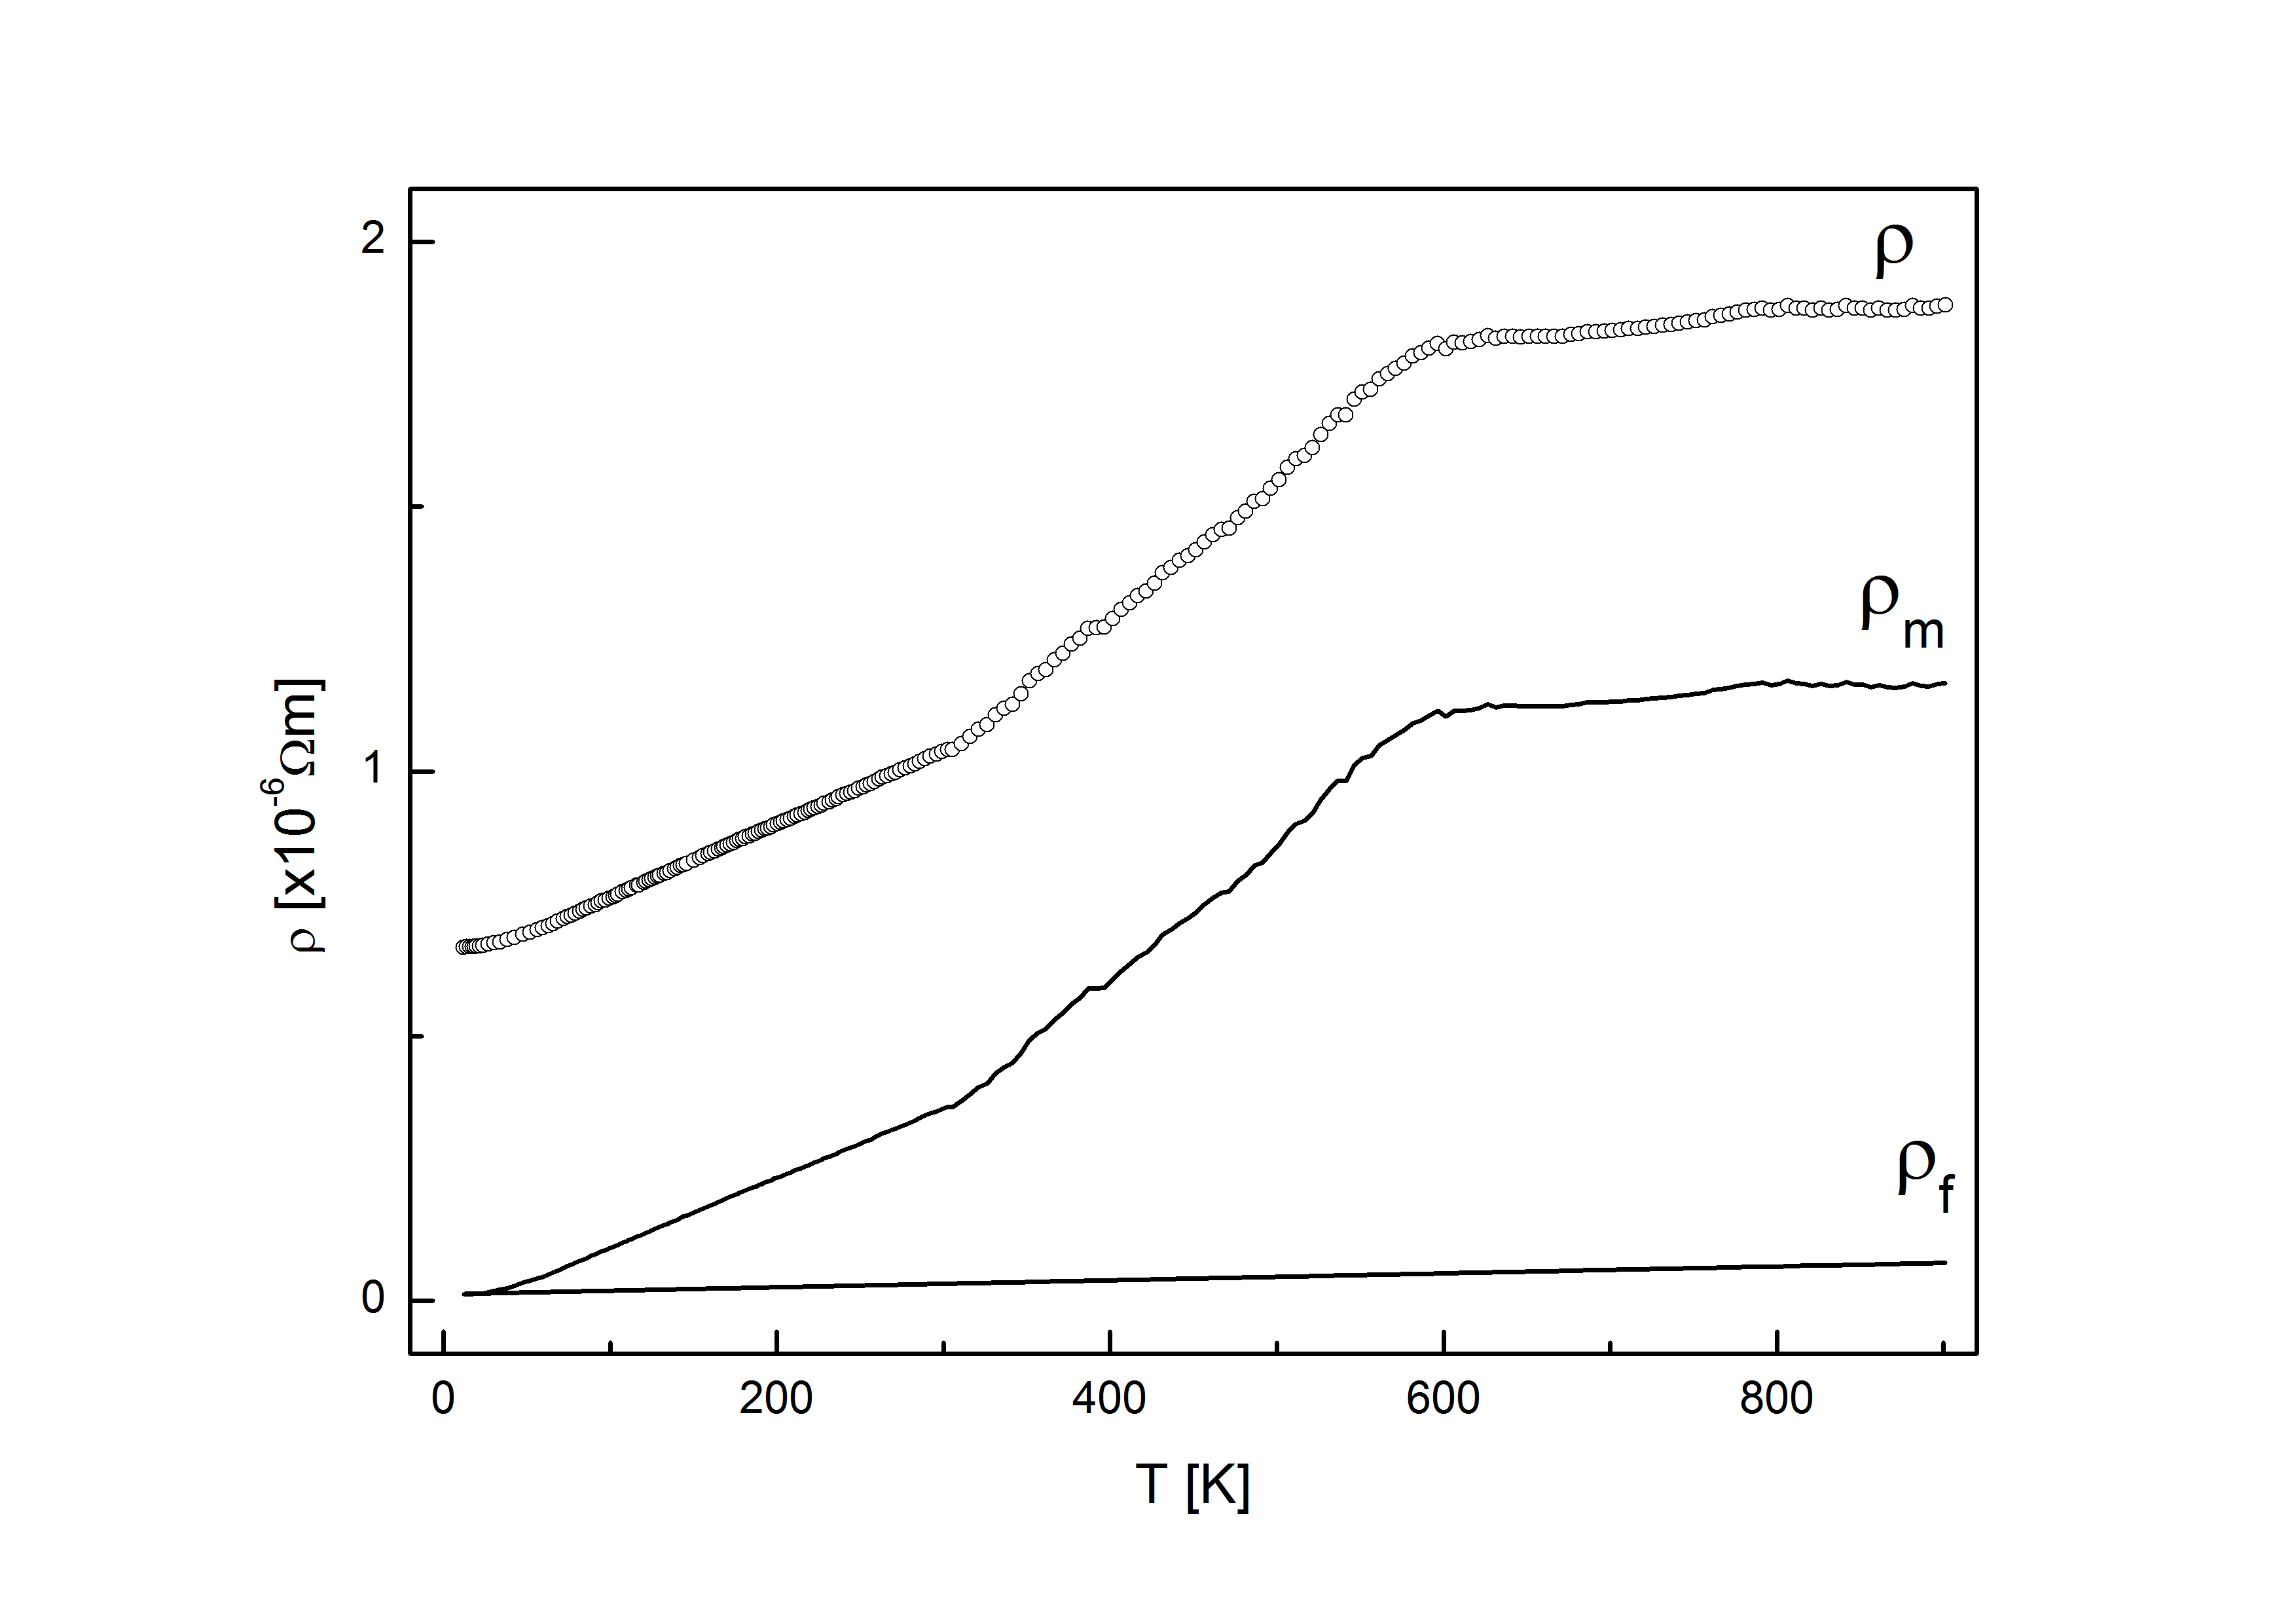
\includegraphics[width =0.85\textwidth]{../img/opor/skladoweDy}
    \caption{Zależność oporności właściwej $\rho$, oporności $\rho_f$ i $\rho_m$ dla $DyFe_2$}
    \label{skladoweDy}
\end{figure}

\begin{figure}[ht]
    \centering
    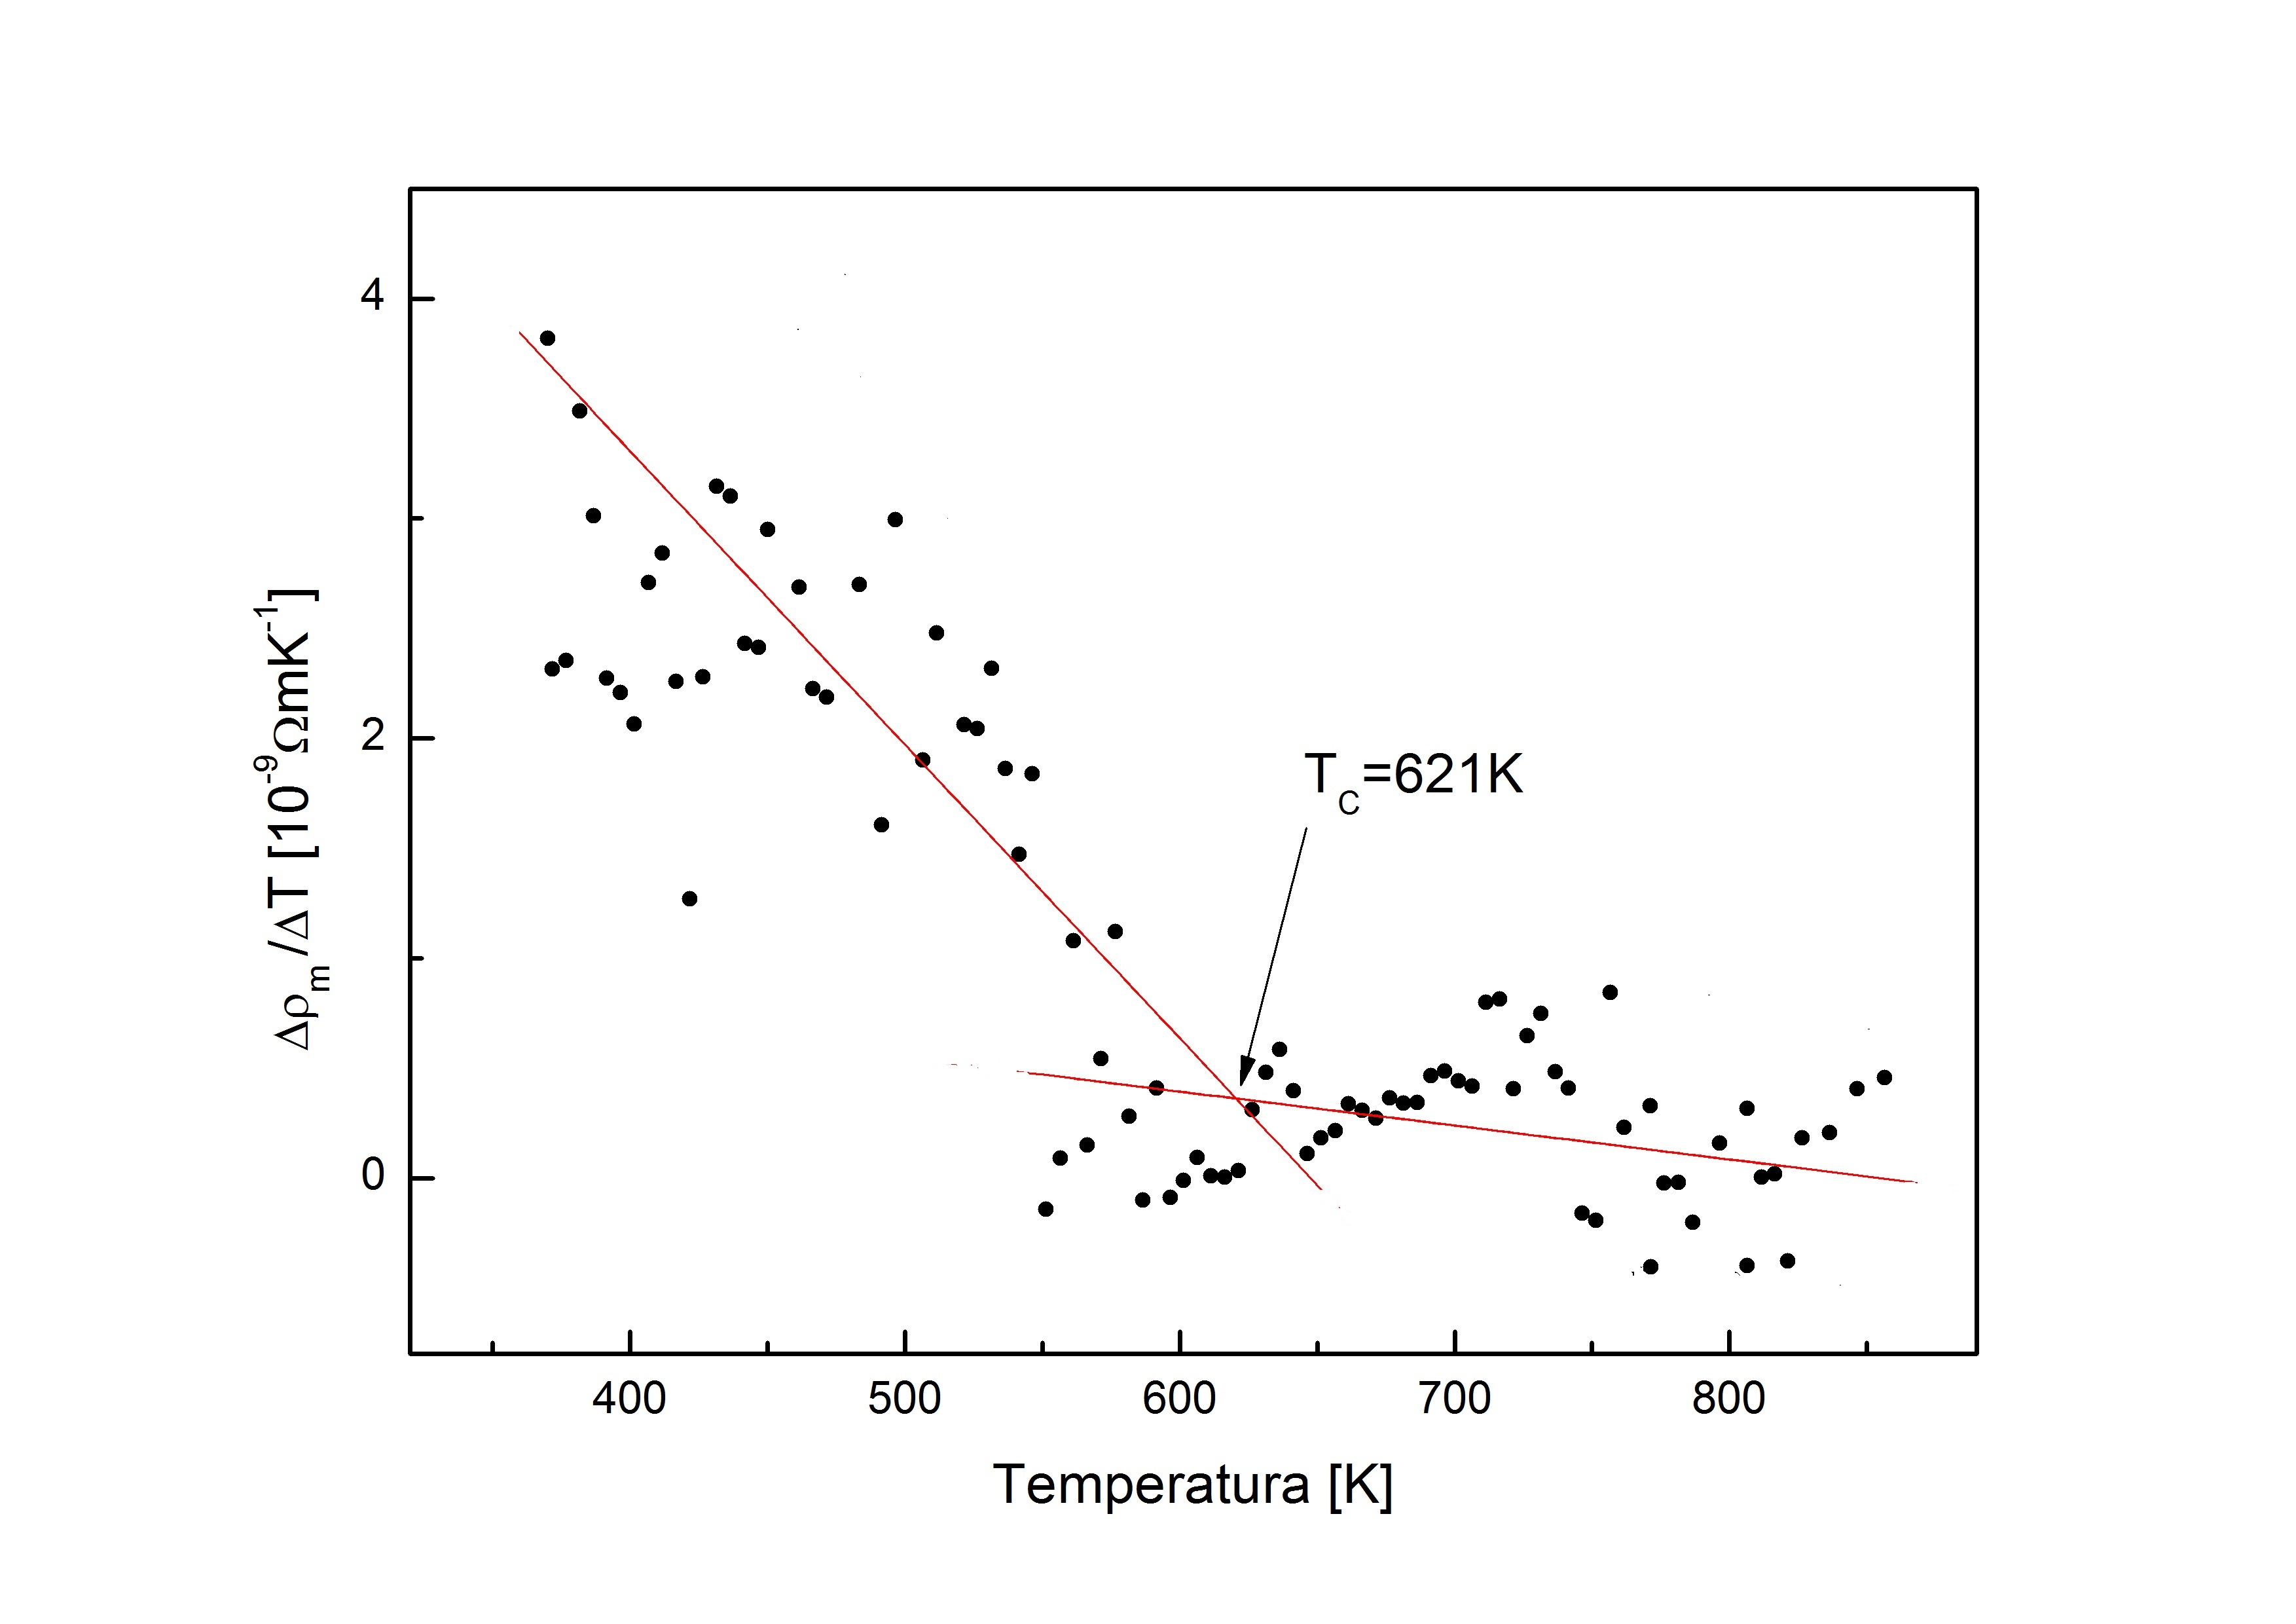
\includegraphics[width =0.8\textwidth]{../img/opor/pochodnaDy}
    \caption{Zależność $\frac{\Delta\rho_m(T)}{\Delta T}$ wraz z wyznaczoną temperaturą Curie $T_C$ dla $DyFe_2$}
    \label{skladoweDy}
\end{figure}

%-----------------------------------------Gd-------------------------------------------------


\begin{figure}[ht]
    \centering
    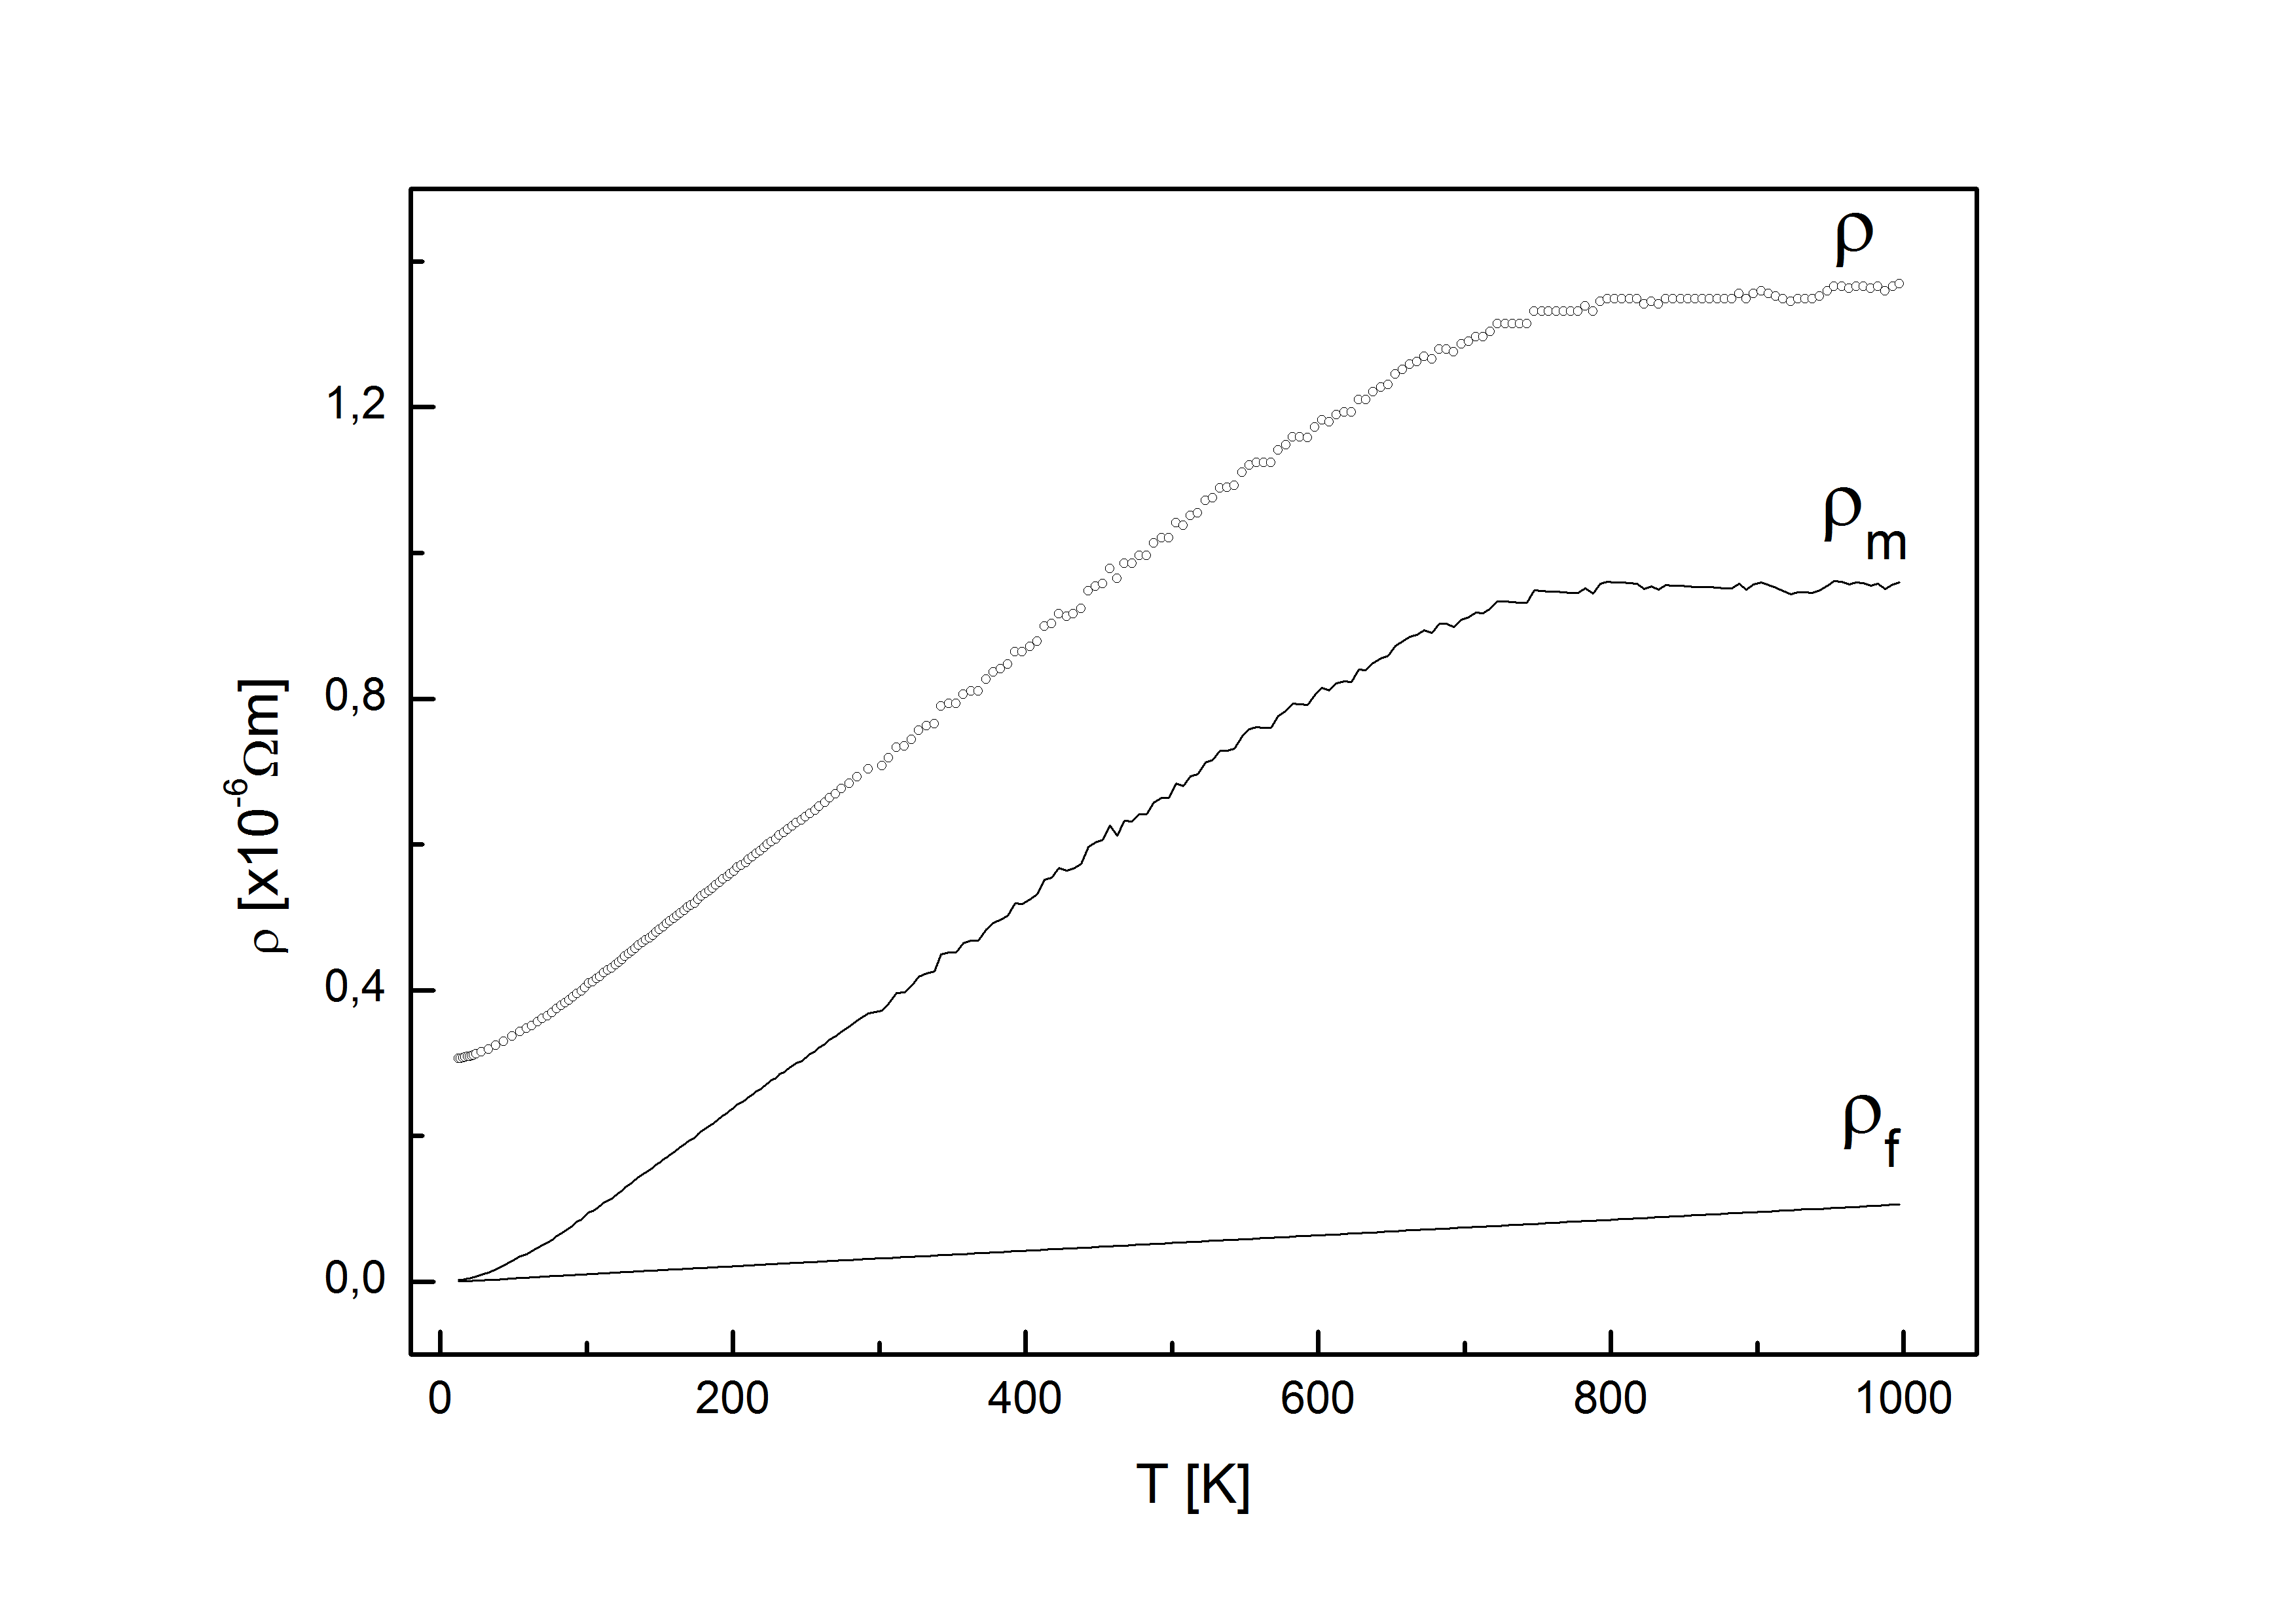
\includegraphics[width =0.8\textwidth]{../img/opor/skladoweGd}
    \caption{Zależność oporności właściwej $\rho$, oporności $\rho_f$ i $\rho_m$ dla $GdFe_2$}
    \label{skladoweGd}
\end{figure}

\begin{figure}[ht]
    \centering
    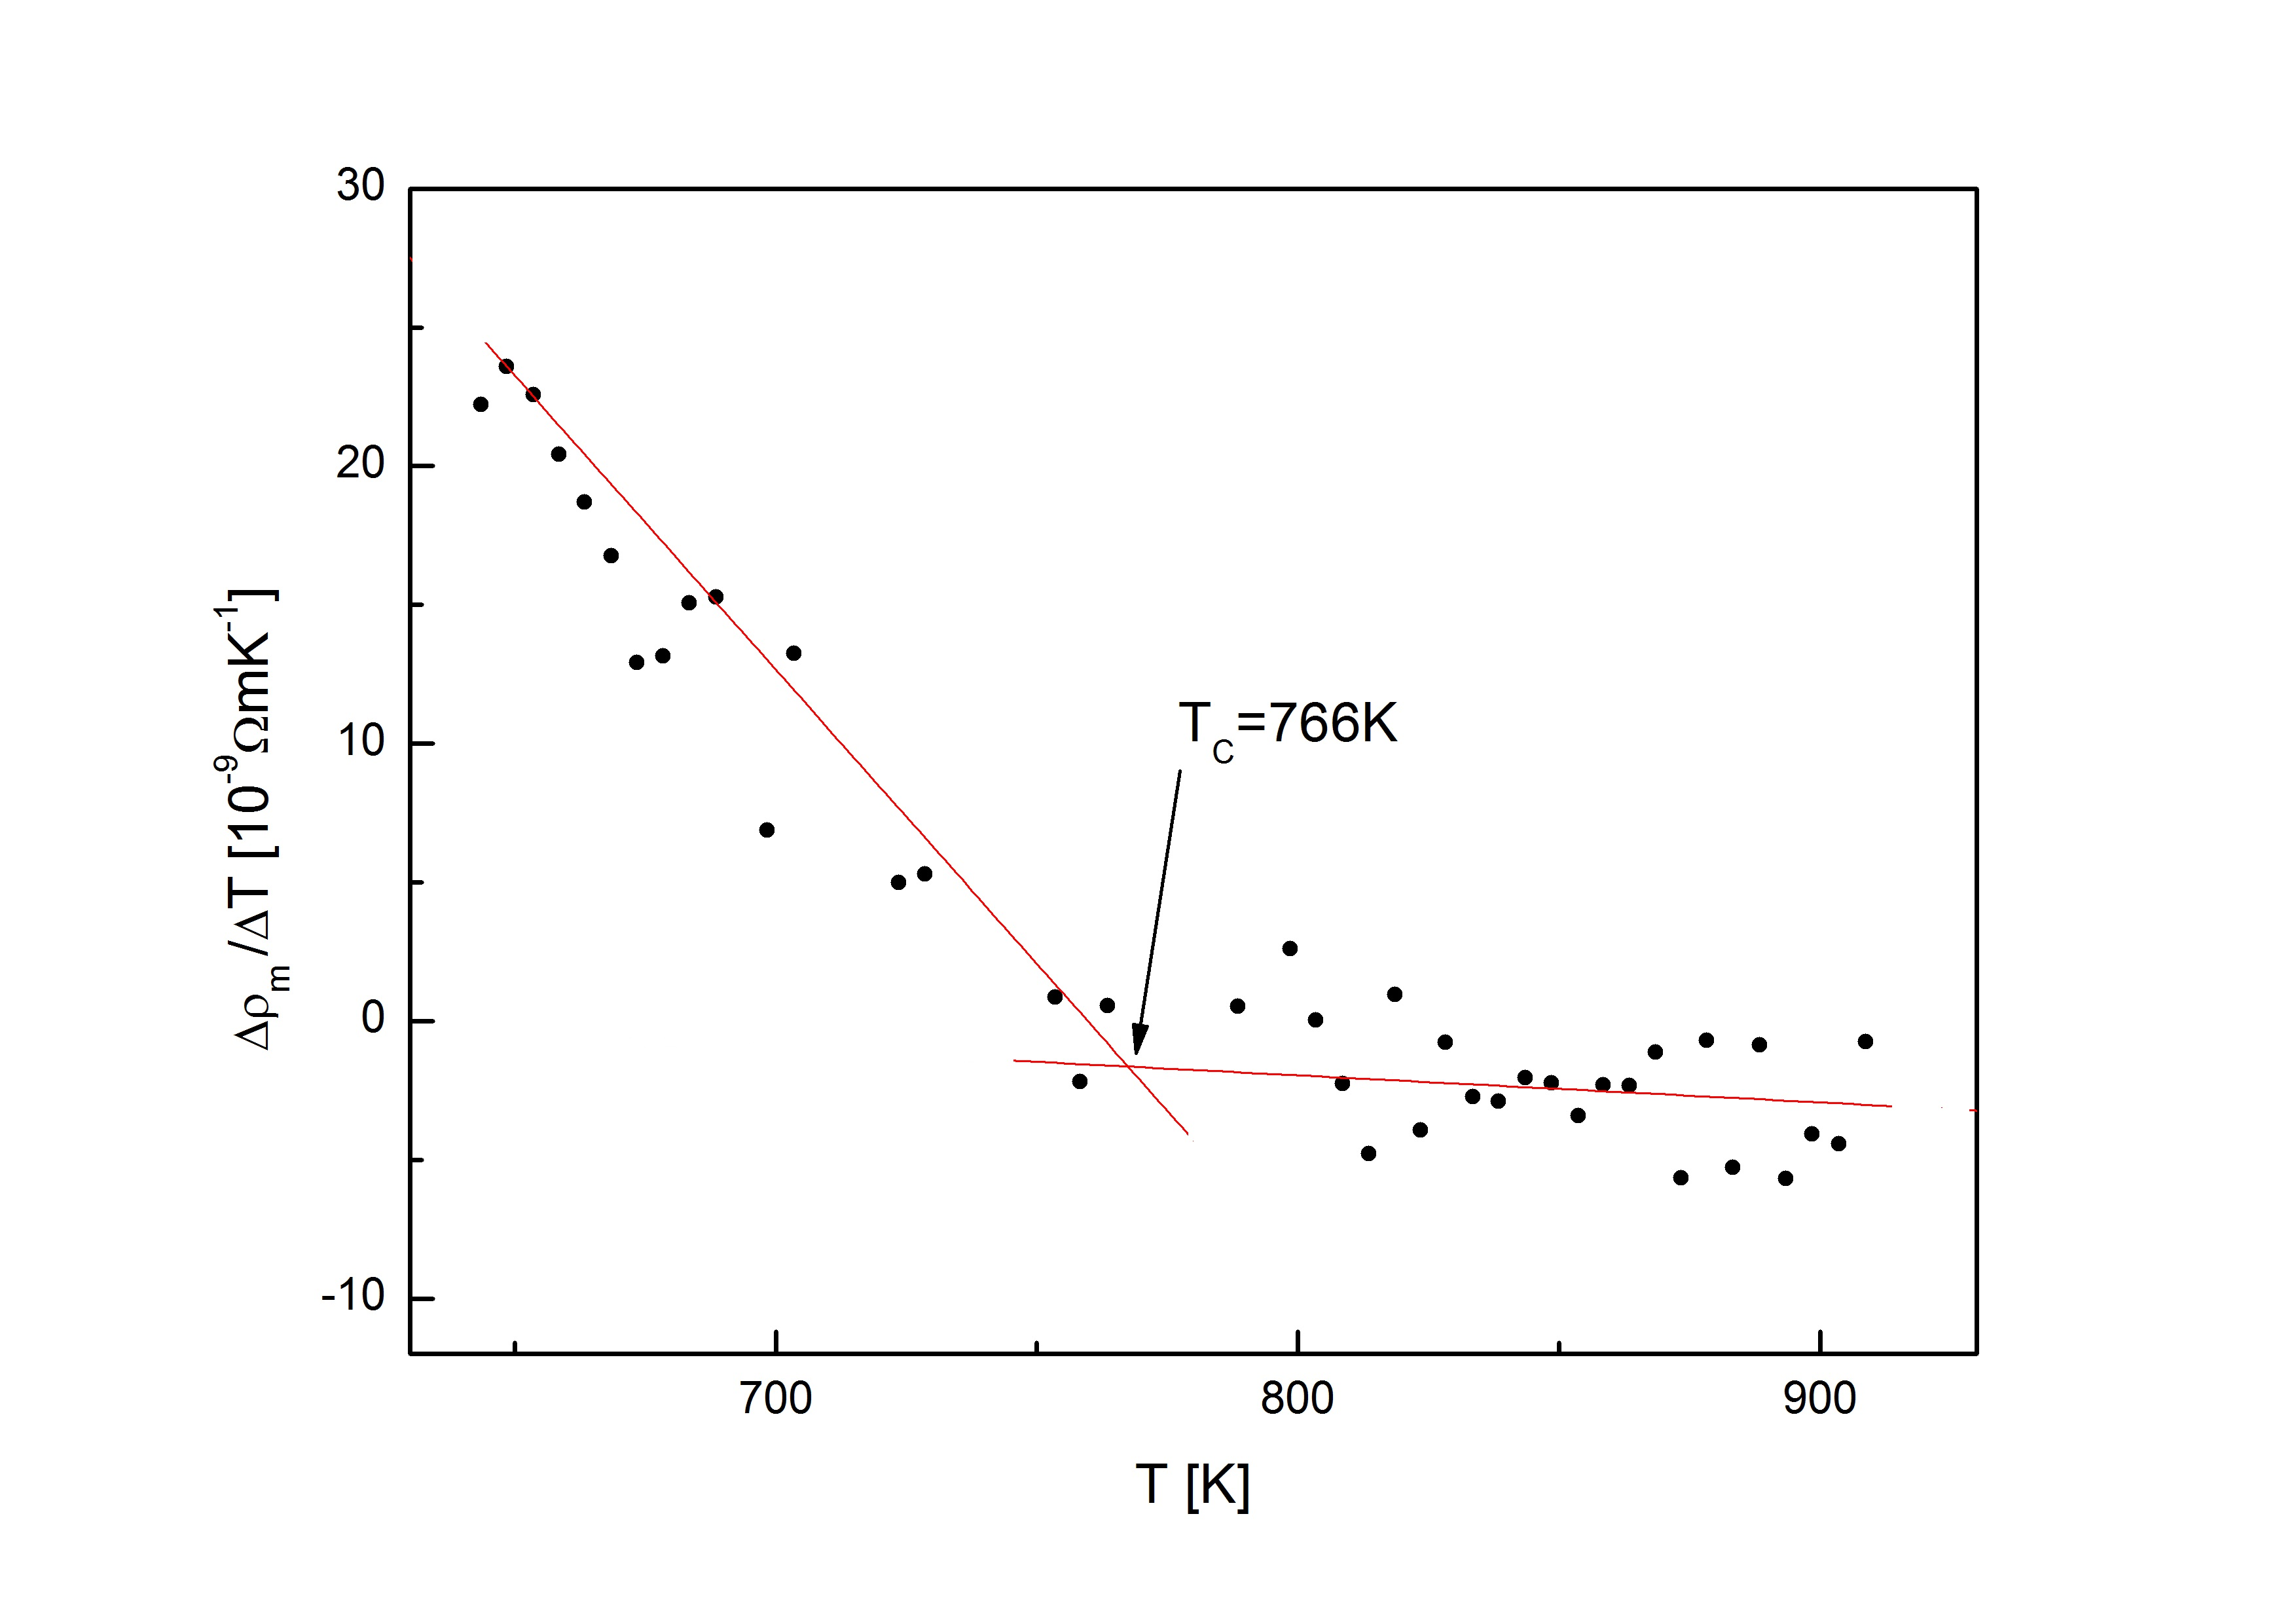
\includegraphics[width =0.8\textwidth]{../img/opor/pochodnaGd}
    \caption{Zależność $\frac{\Delta\rho_m(T)}{\Delta T}$ wraz z wyznaczoną temperaturą Curie $T_C$ dla $GdFe_2$}
    \label{skladoweGd}
\end{figure}


%-----------------------------------------Ho-------------------------------------------------


\begin{figure}[ht]
    \centering
    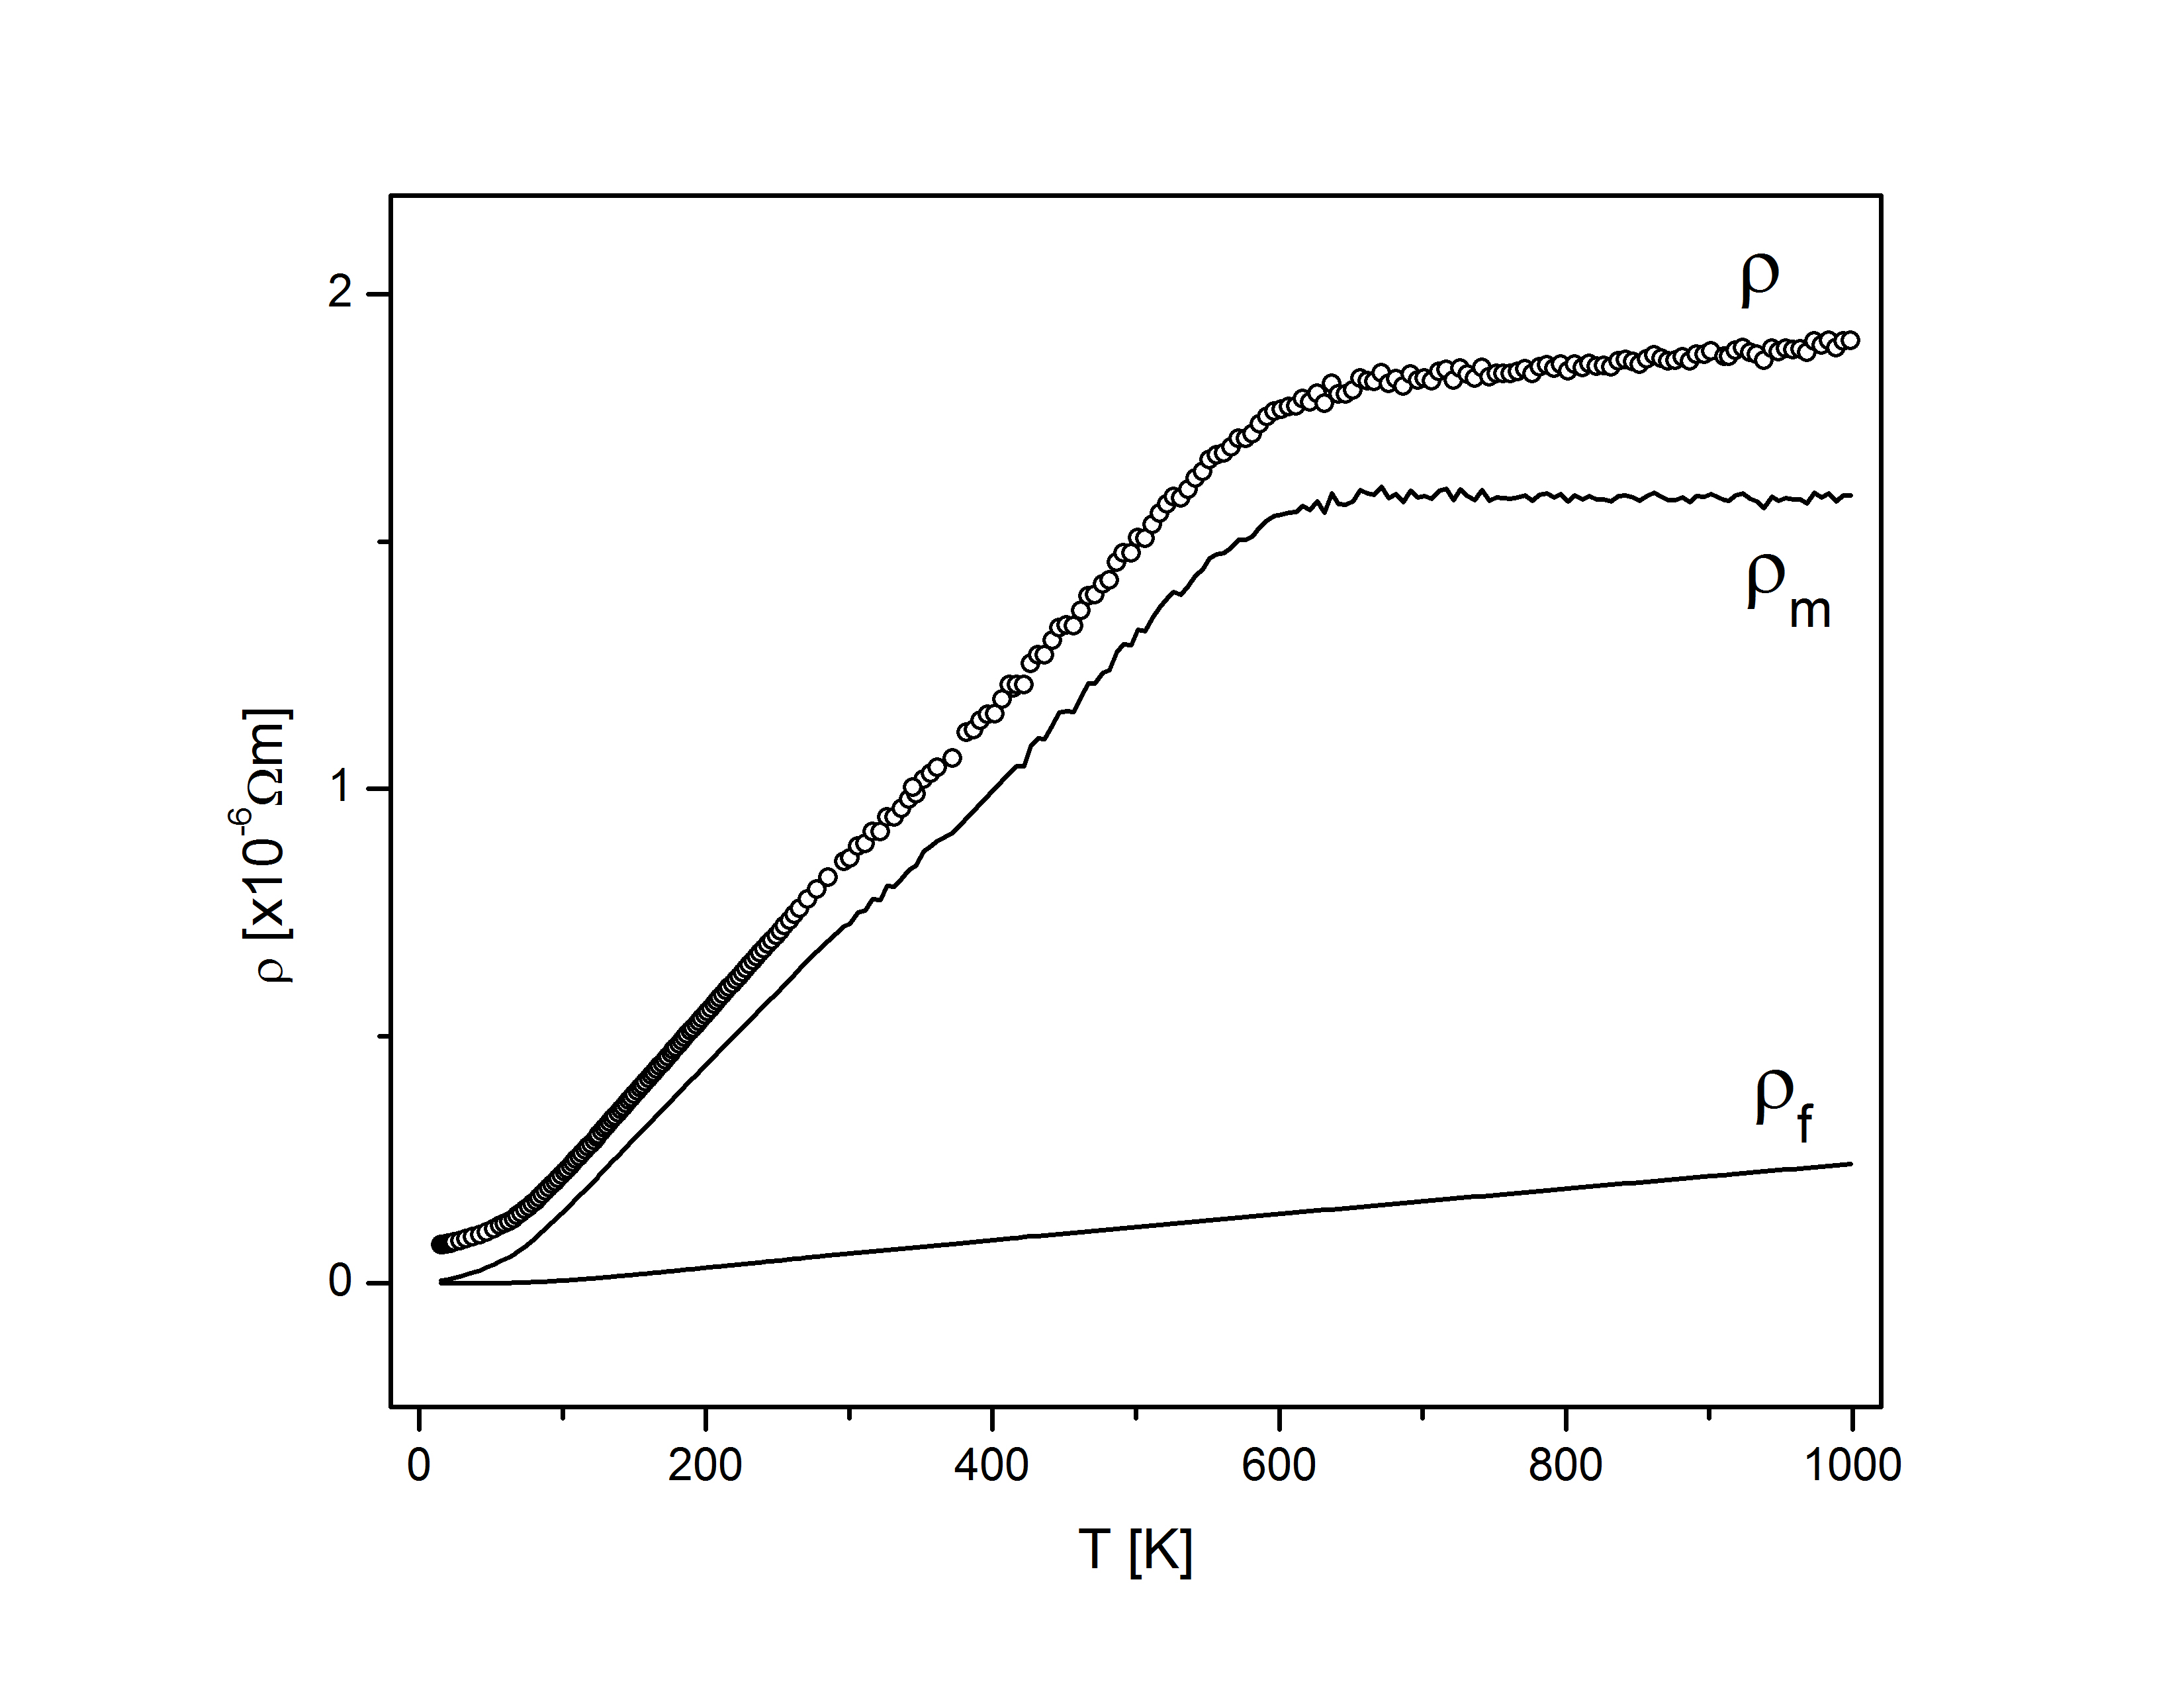
\includegraphics[width =0.8\textwidth]{../img/opor/skladoweHo}
    \caption{Zależność oporności właściwej $\rho$, oporności $\rho_f$ i $\rho_m$ dla $HoFe_2$}
    \label{skladoweHo}
\end{figure}

\begin{figure}[ht]
    \centering
    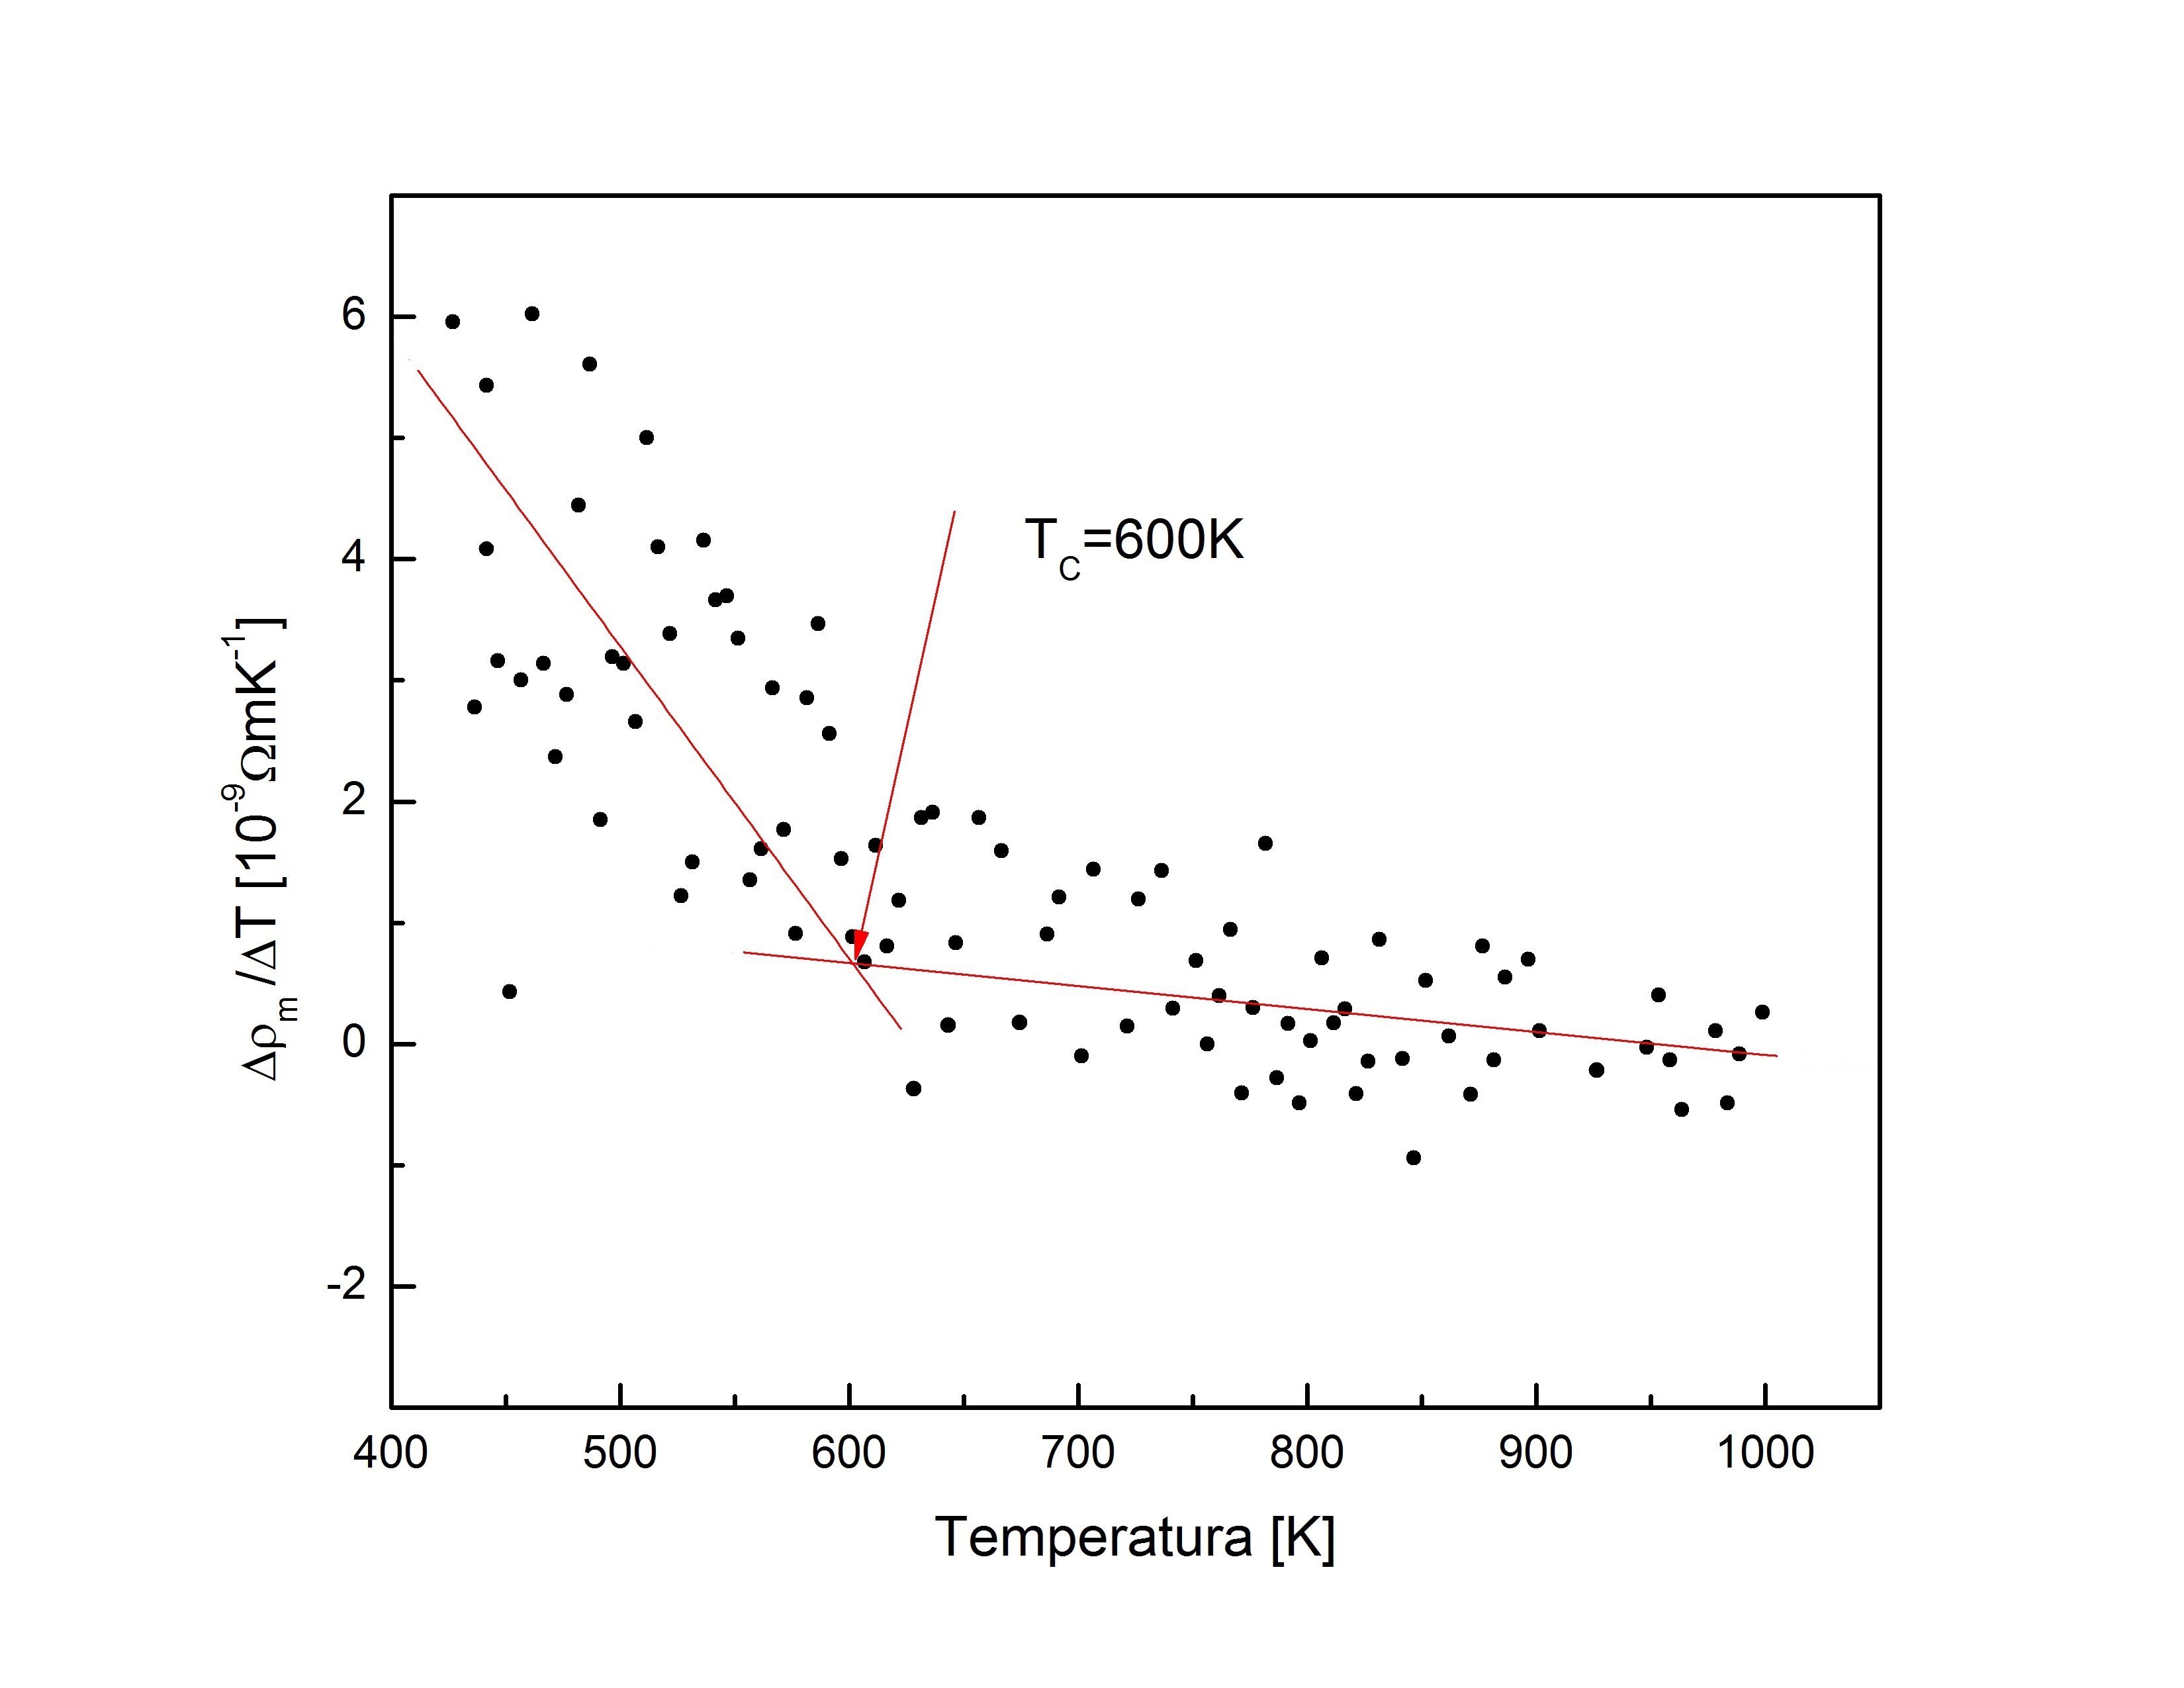
\includegraphics[width =0.8\textwidth]{../img/opor/pochodnaHo}
    \caption{Zależność $\frac{\Delta\rho_m(T)}{\Delta T}$ wraz z wyznaczoną temperaturą Curie $T_C$ dla $HoFe_2$}
    \label{skladoweHo}
\end{figure}


%-----------------------------------------Tb-------------------------------------------------


\begin{figure}[ht]
    \centering
    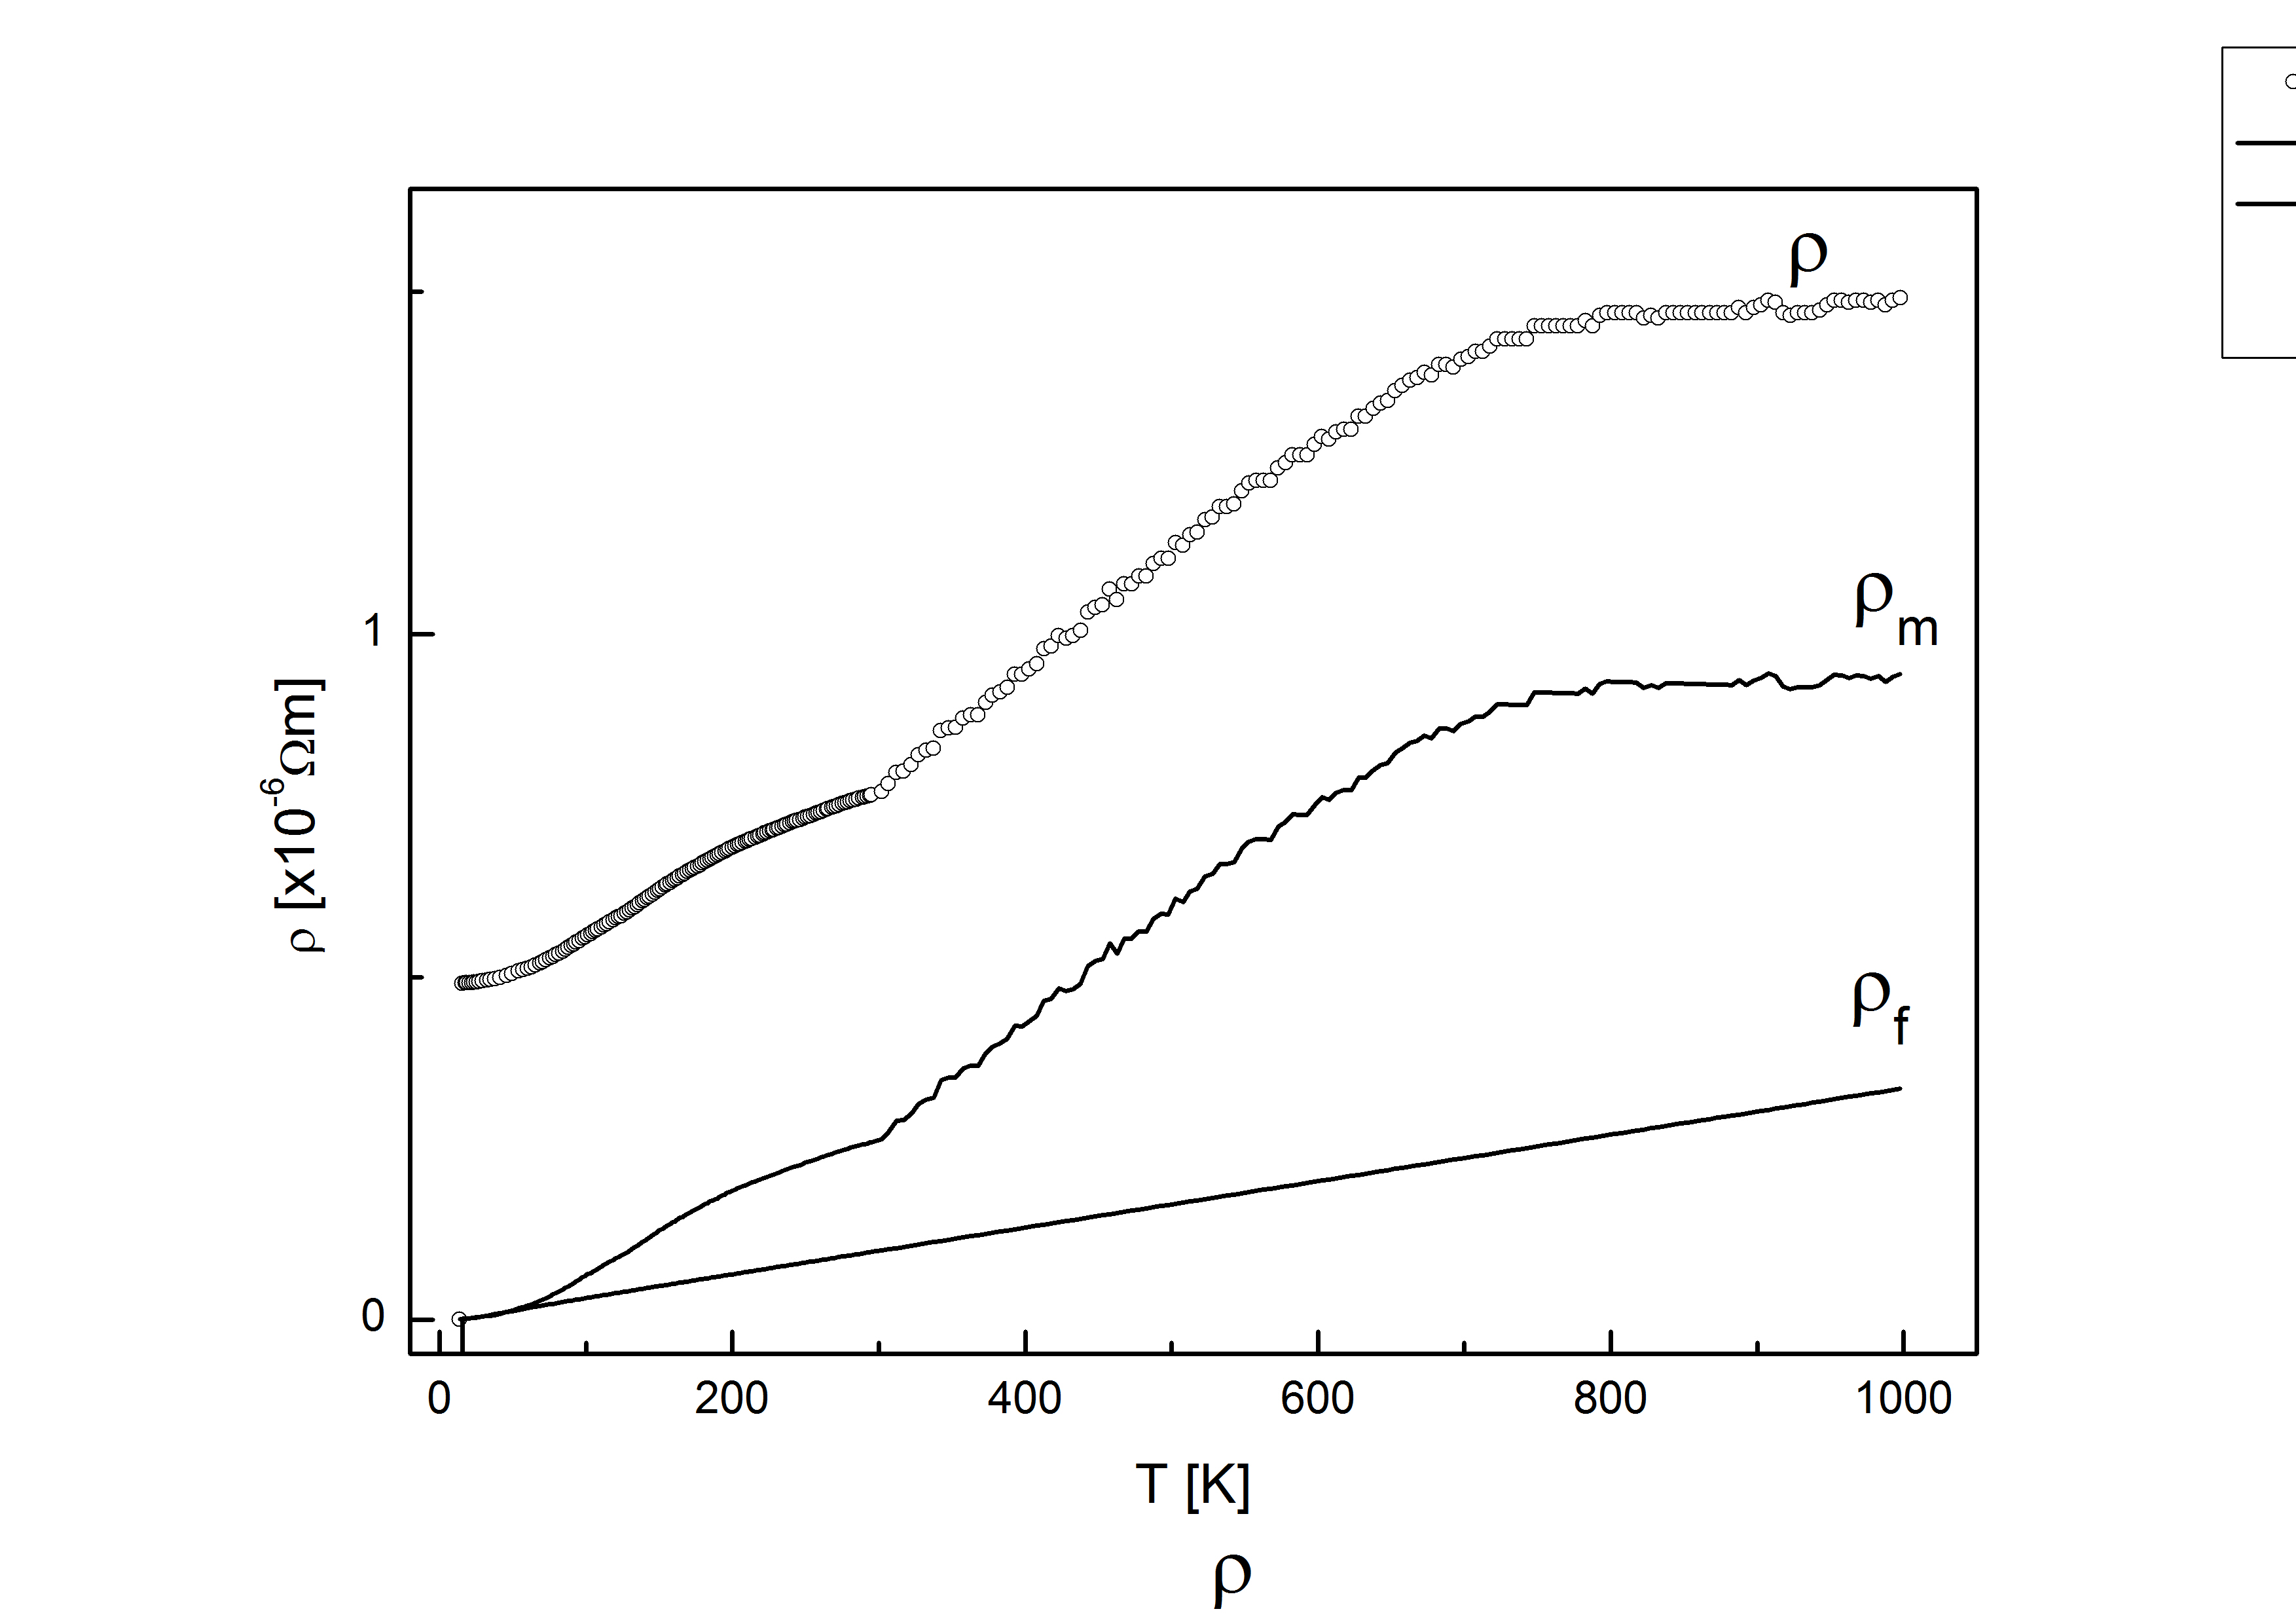
\includegraphics[width =0.8\textwidth]{../img/opor/skladoweTb}
    \caption{Zależność oporności właściwej $\rho$, oporności $\rho_f$ i $\rho_m$ dla $TbFe_2$}
    \label{skladoweTb}
\end{figure}

\begin{figure}[ht]
    \centering
    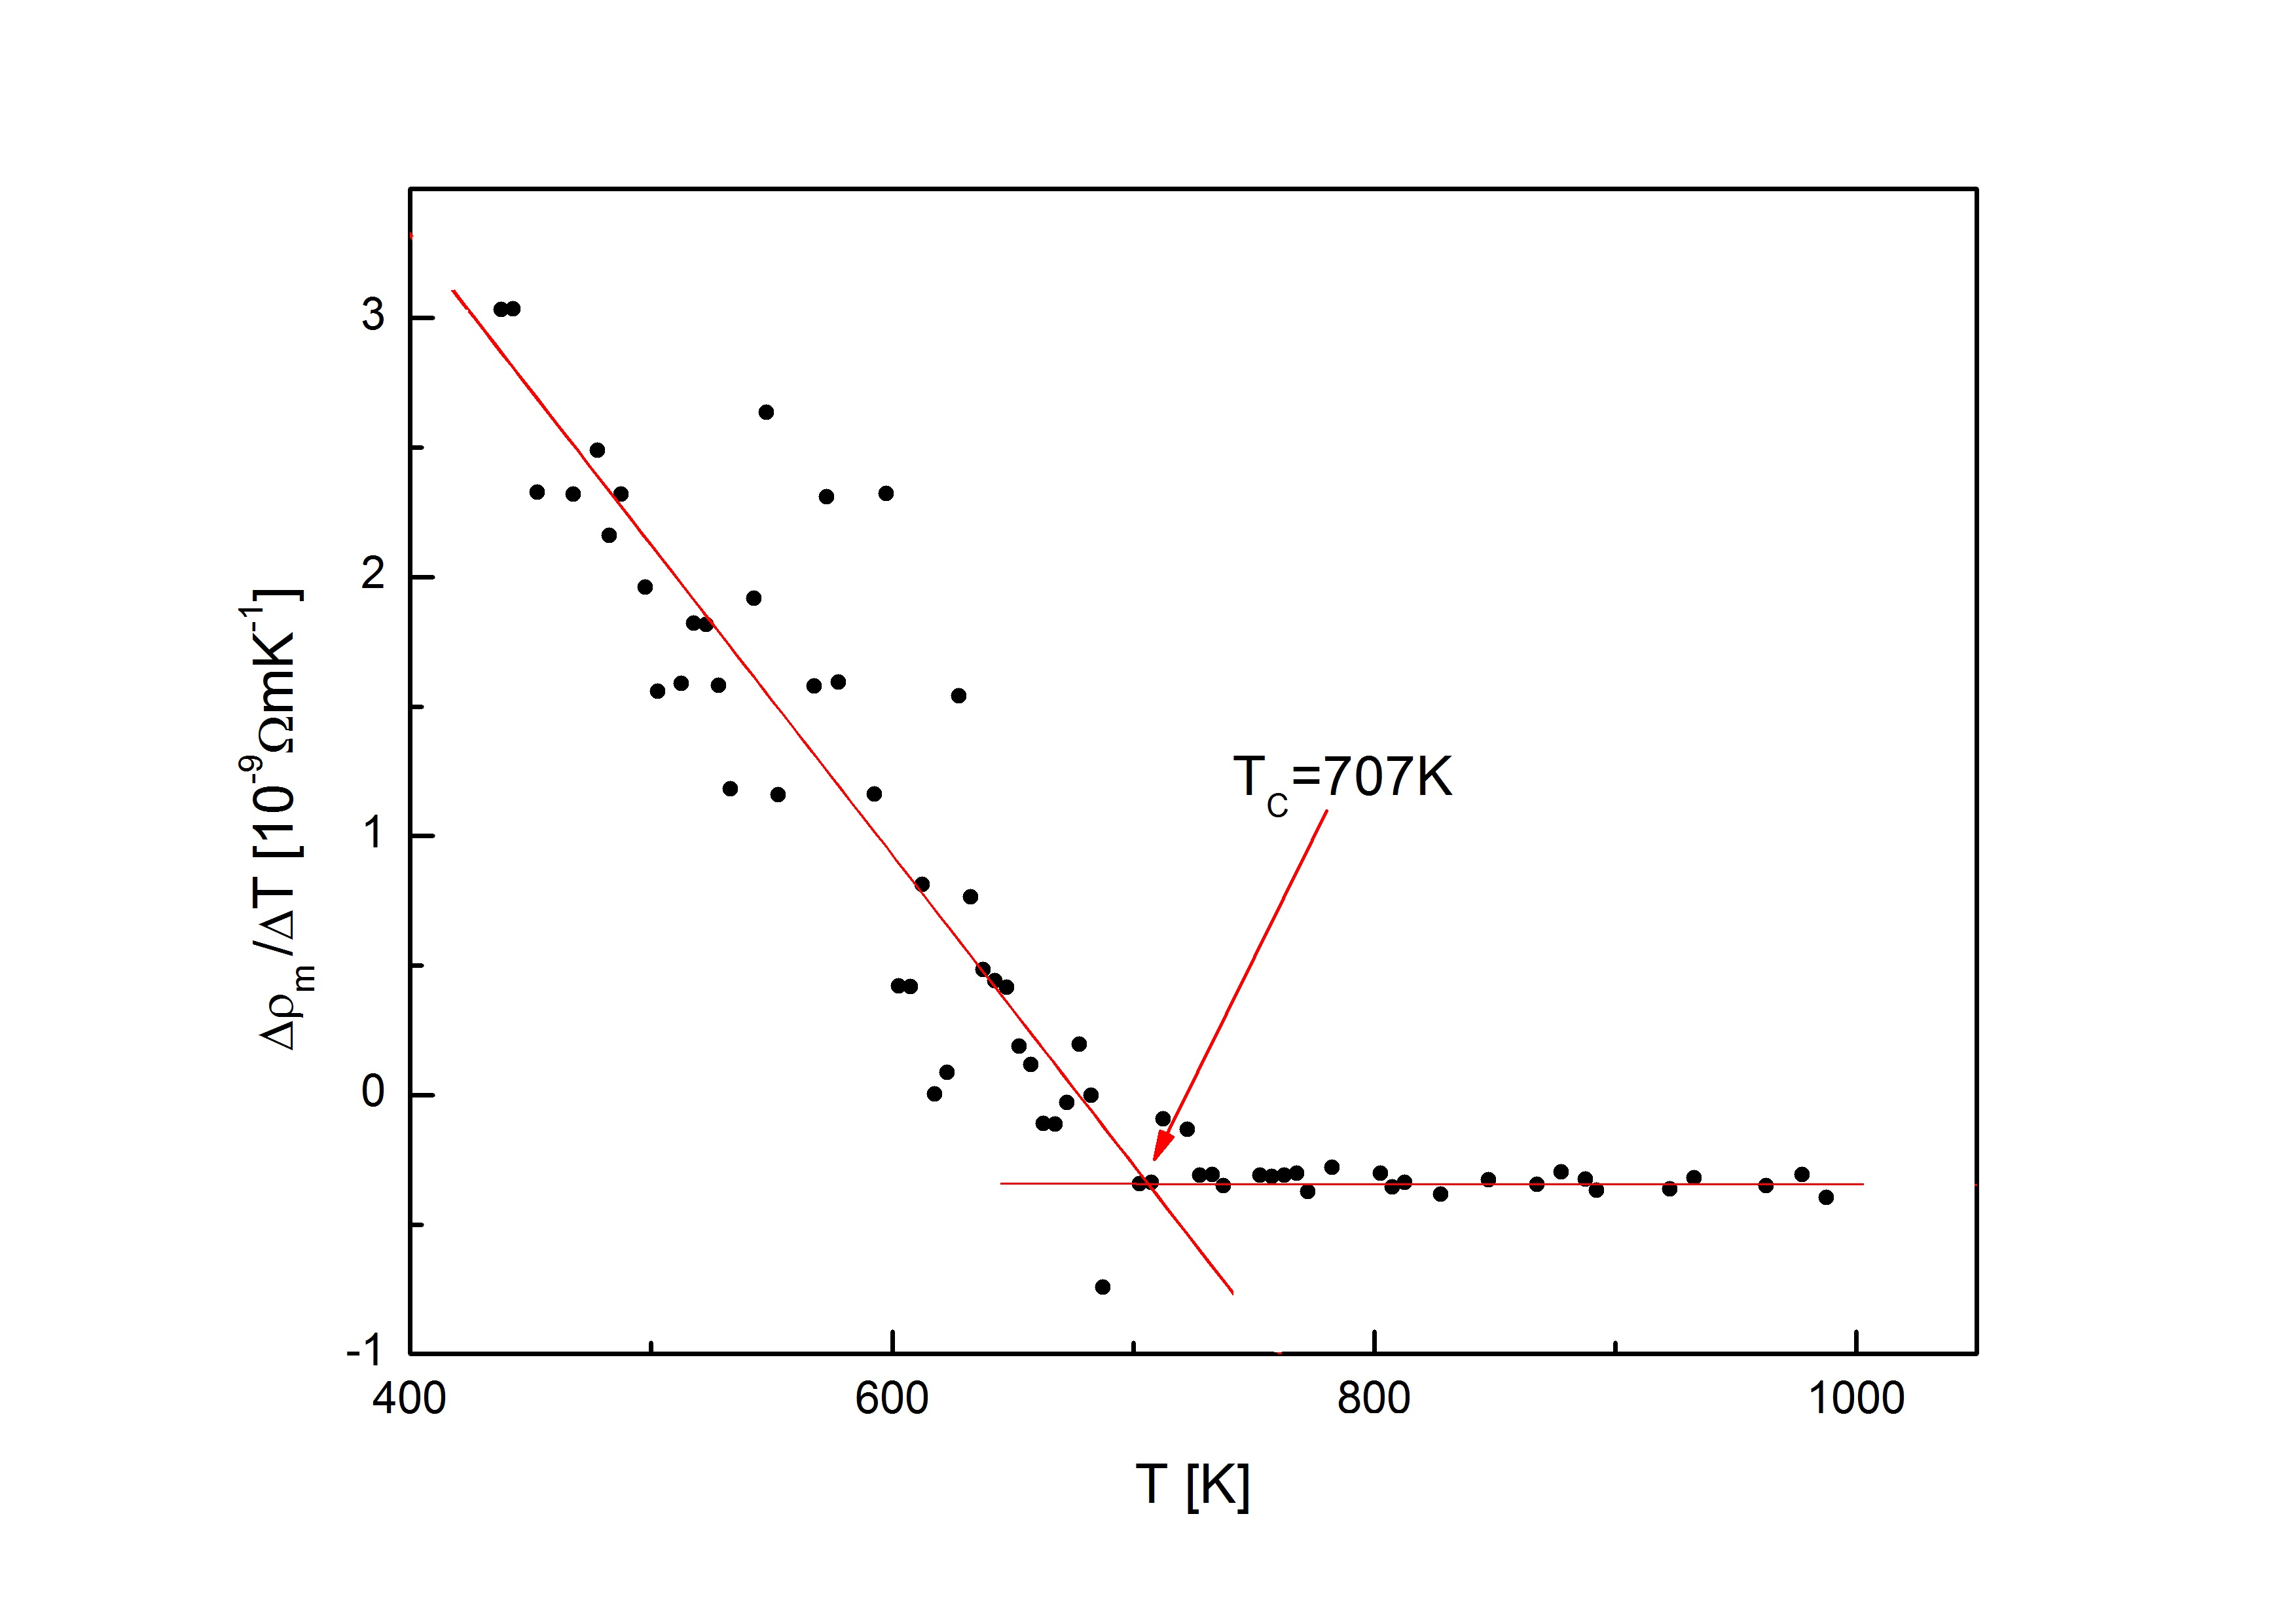
\includegraphics[width =0.8\textwidth]{../img/opor/pochodnaTb}
    \caption{Zależność $\frac{\Delta\rho_m(T)}{\Delta T}$ wraz z wyznaczoną temperaturą Curie $T_C$ dla $TbFe_2$}
    \label{skladoweTb}
\end{figure}


%-----------------------------------------Y-------------------------------------------------


\begin{figure}[ht]
    \centering
    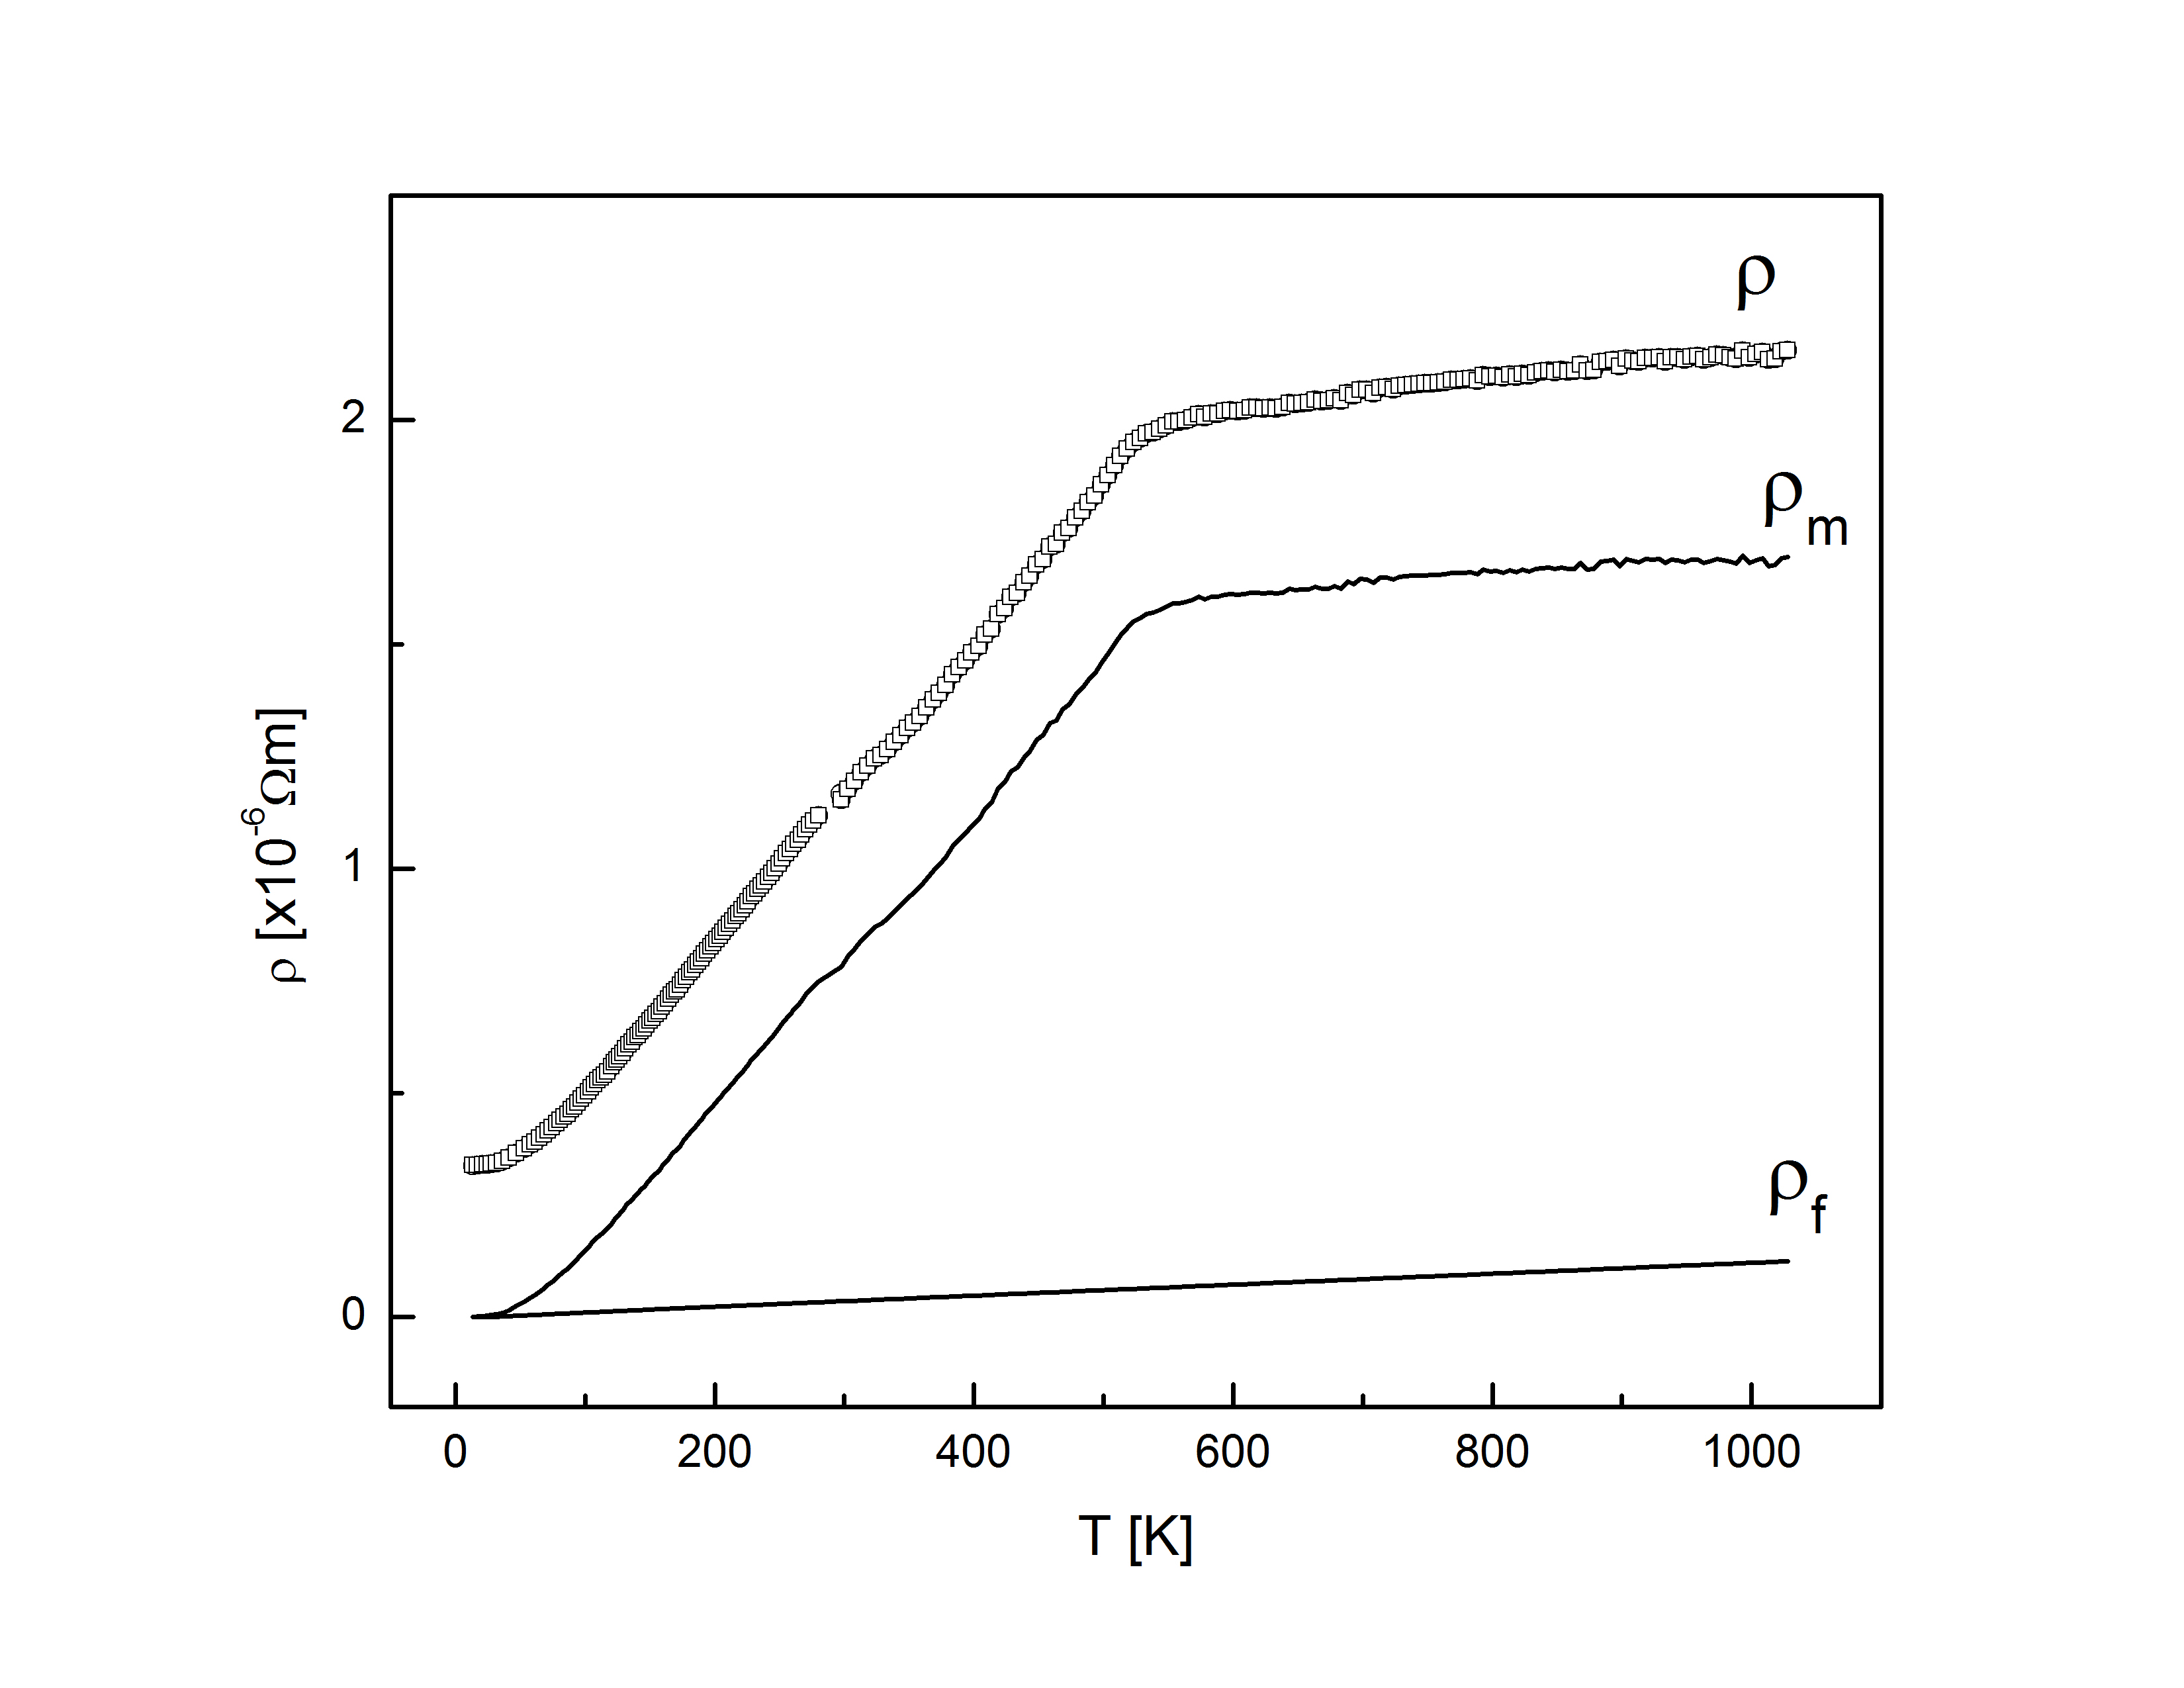
\includegraphics[width =0.8\textwidth]{../img/opor/skladoweY}
    \caption{Zależność oporności właściwej $\rho$, oporności $\rho_f$ i $\rho_m$ dla $YFe_2$}
    \label{skladoweY}
\end{figure}

\begin{figure}[ht]
    \centering
    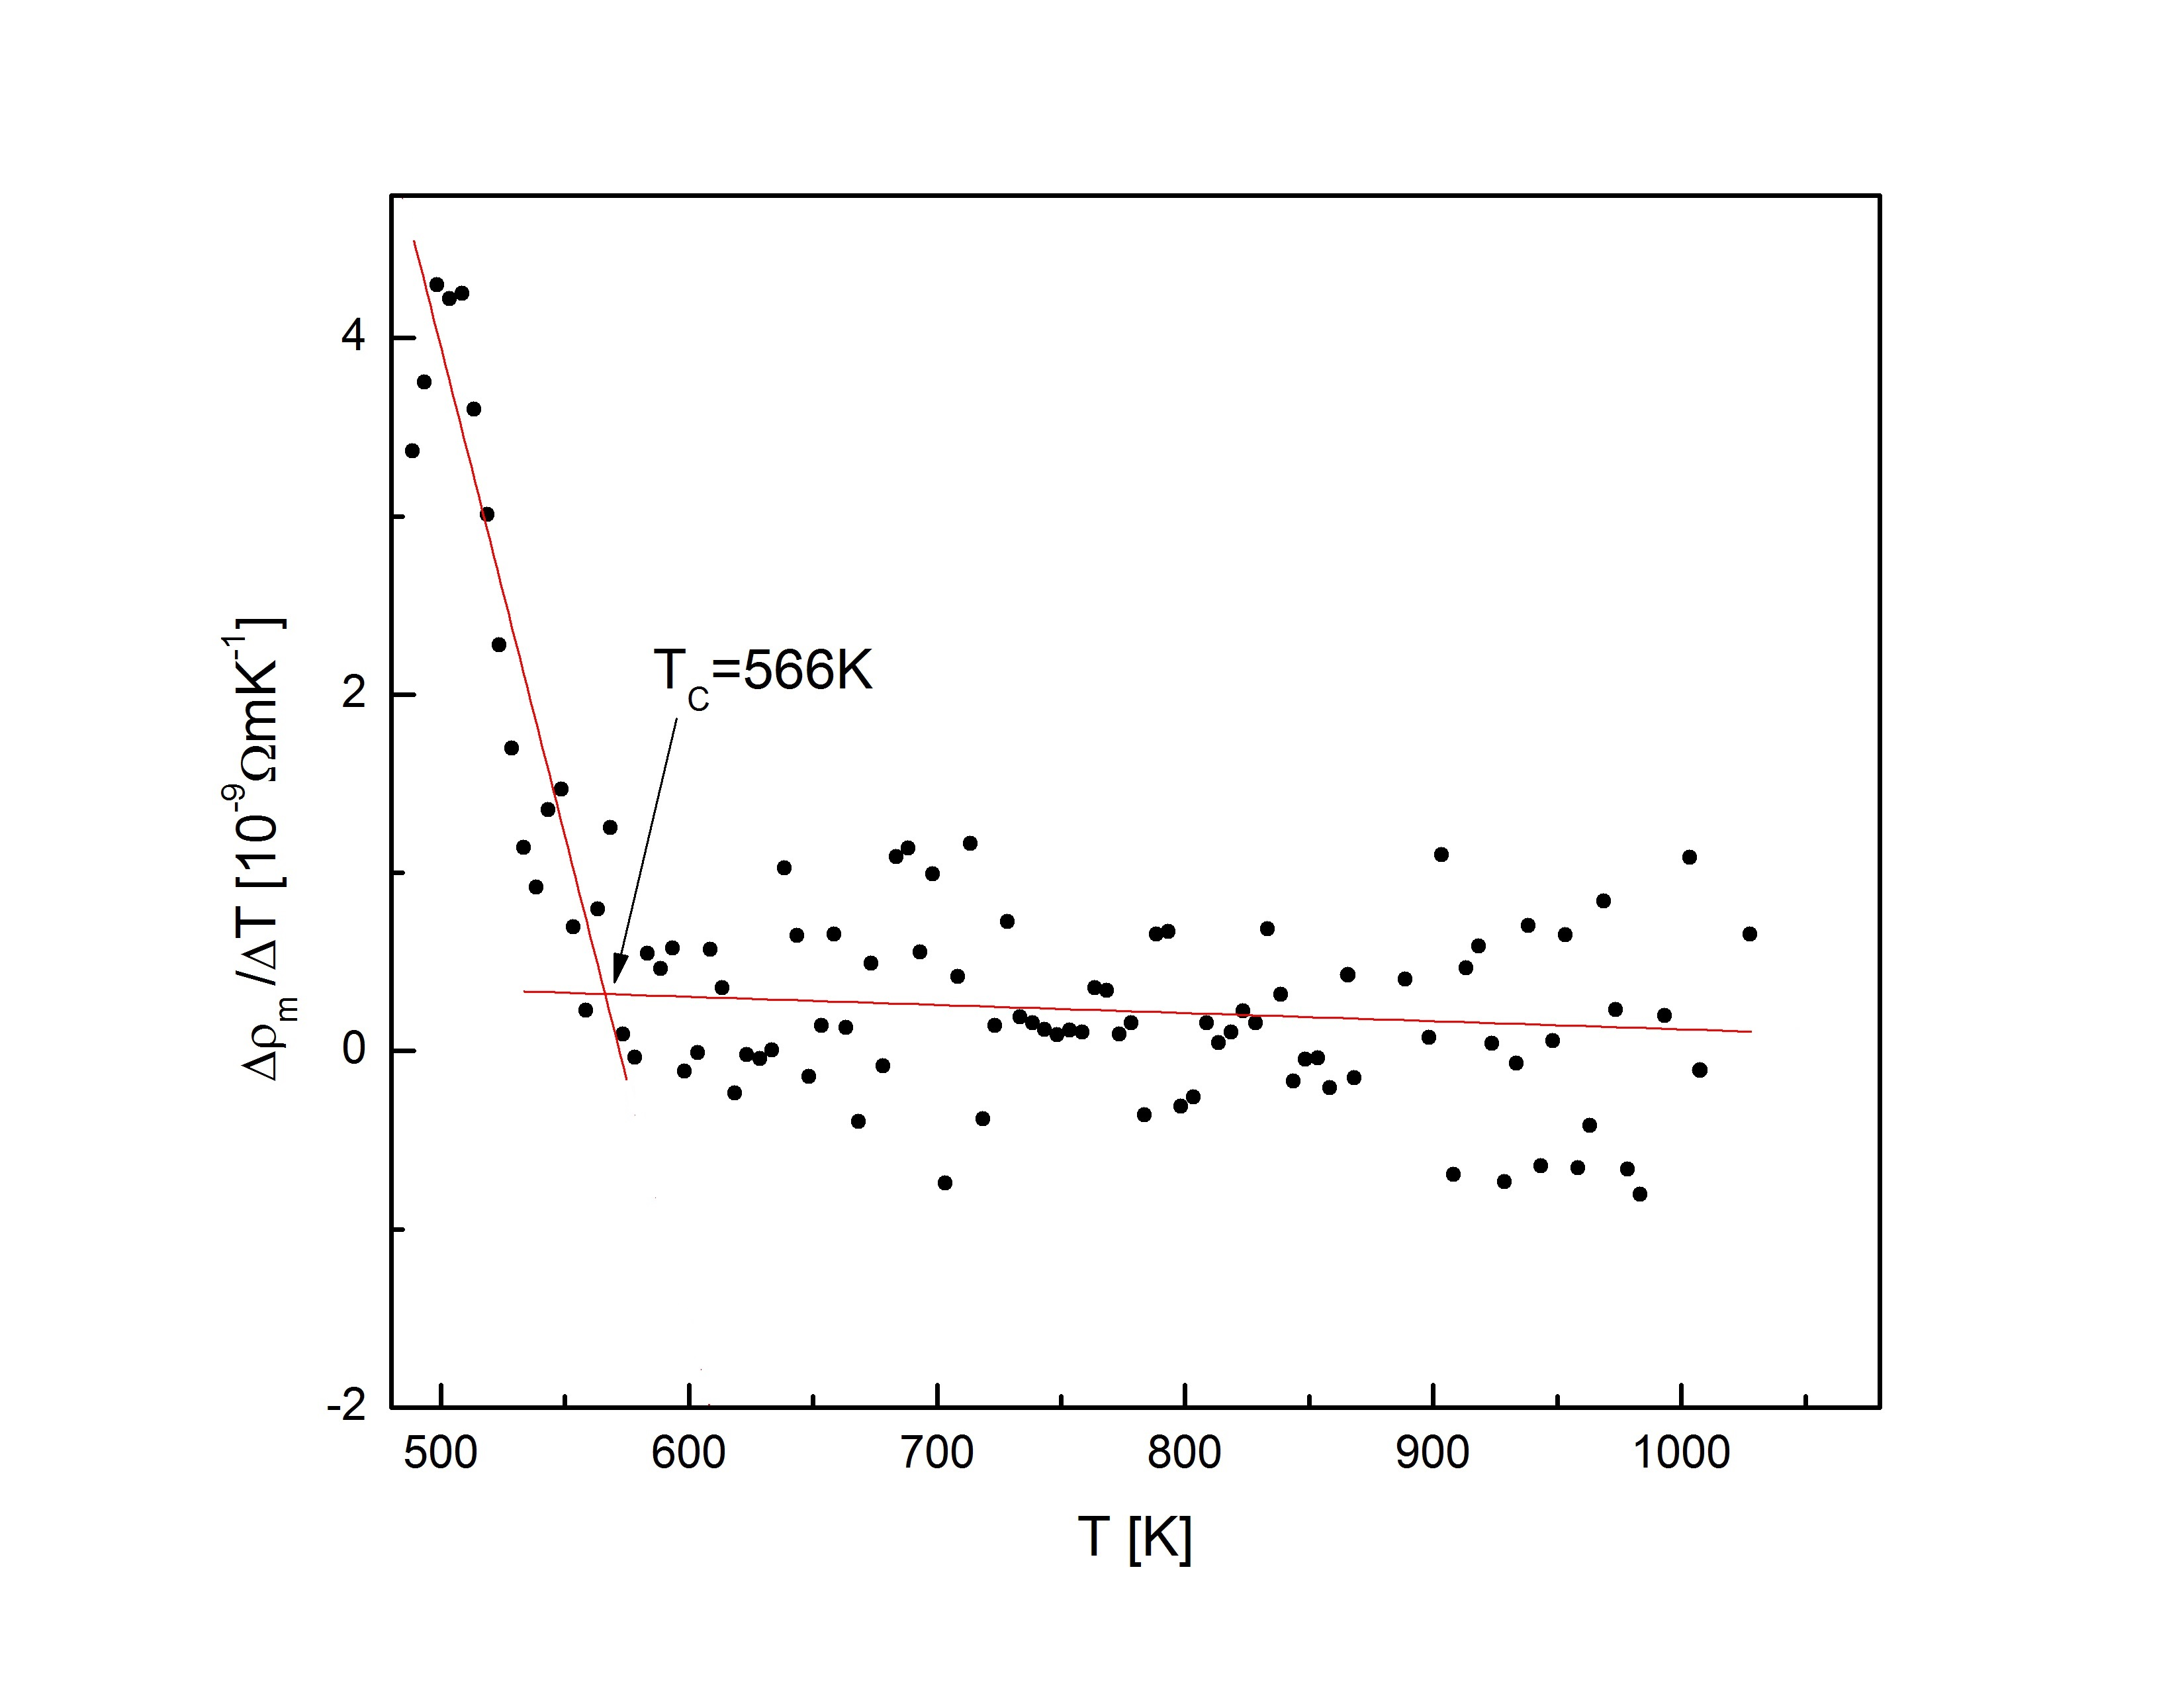
\includegraphics[width =0.8\textwidth]{../img/opor/pochodnaY}
    \caption{Zależność $\frac{\Delta\rho_m(T)}{\Delta T}$ wraz z wyznaczoną temperaturą Curie $T_C$ dla $YFe_2$}
    \label{skladoweY}
\end{figure}


%-----------------------------------------------------------------
%-------------------Parametry oporności---------------------
%-----------------------------------------------------------------
\clearpage
\subsection{Parametry oporności właściwej badanych próbek}

Zebrane dane pomiarowe posłużyły do wyznaczenia wielkości o których była mowa w części teoretycznej. Wartości te zostały zebrane w tabeli \ref{tabParametryOpor}

  \begin{table}[ht]
  \centering
  \footnotesize
  \caption{Wartości wyznaczone na podstawie pomiarów oporności elektrycznej}
  \label{tabParametryOpor}
  \begin{tabular}{|c|c|c|c|c|c|c|c|c|}
    \hline
Związek	&	$\rho_0$	&	$\theta_D$	&	$\rho_{m\infty}$	&	$A_2 $	&	$A_1$	&	$A_3$	&	$R_t $	&	$T_C$ \\
	&	$[10^{-6}{\Omega}m]$	&	$[K]$	&	$ [10^{-6}{\Omega}m]$	&	$ [10^{-6}{\Omega}m/K^2]$	&	$[10^{-6}{\Omega}m/K]$	&	$ [10^{-6}{\Omega}m]$	&	$ [10^{-6}{\Omega}m]$	&	$[K]$		\\\hline
$YFe_2$	&	0,33618	&	168	&	1,694210	&	4,17E+00	&	3,40E+00	&	1,21E-04	&	2,04E-02	&	566	\\\hline
$GdFe_2$	&	0,30418	&	105	&	0,959710	&	4,53E-06	&	8,01E-05	&	1,05E-04	&	1,12E-02	&	766	\\\hline
$TbFe_2$	&	0,48907	&	129	&	0,941520	&	7,81E-08	&	9,91E-09	&	6,06E-05	&	7,86E-03	&	707	\\\hline
$DyFe_2$	&	0,62482	&	42	&	1,166223	&	3,28E-04	&	7,30E-03	&	6,54E-05	&	2,78E-03	&	621	\\\hline
$HoFe_2$	&	0,07195	&	588	&	0,241430	&	1,03E+00	&	2,01E+00	&	2,46E-04	&	1,45E-01	&	600	\\\hline
  \end{tabular}
\end{table}

Otrzymane wartości temperatury Curie badanych związków porównano z wartościami literaturowymi. Wyniki zamieszczono w tabeli \ref{tabTCurie} oraz na wykresie \ref{RysTempCurie}. Kolorem czerwonym zaznaczono punkty pomiarowe, na niebiesko i zielono oznaczono
dane zaczerpnięte kolejno 
z REF DO BIBLIOGRAFIIII. 

  \begin{table}[ht]
  \centering
  \footnotesize
  \caption{Temperatury Curie badanych próbek i wartości literaturowe}
  \label{tabTCurie}
  \begin{tabular}{|c|c|c|c|}
    \hline
Związek	&	Wartości zmierzone [K]	&	Dane literaturowe 1 [K]	&	Dane literaturowe 2 [K]	\\\hline
$YFe_2$	&	566	&	550	&	560	\\\hline
$GdFe_2$	&	766	&	785	&	760	\\\hline
$TbFe_2$	&	707	&	711	&	700	\\\hline
$DyFe_2$	&	621	&	635	&	630	\\\hline
$HoFe_2$	&	600	&	612	&	600	\\\hline  
  \end{tabular}
\end{table}

\begin{figure}[ht]
    \centering
    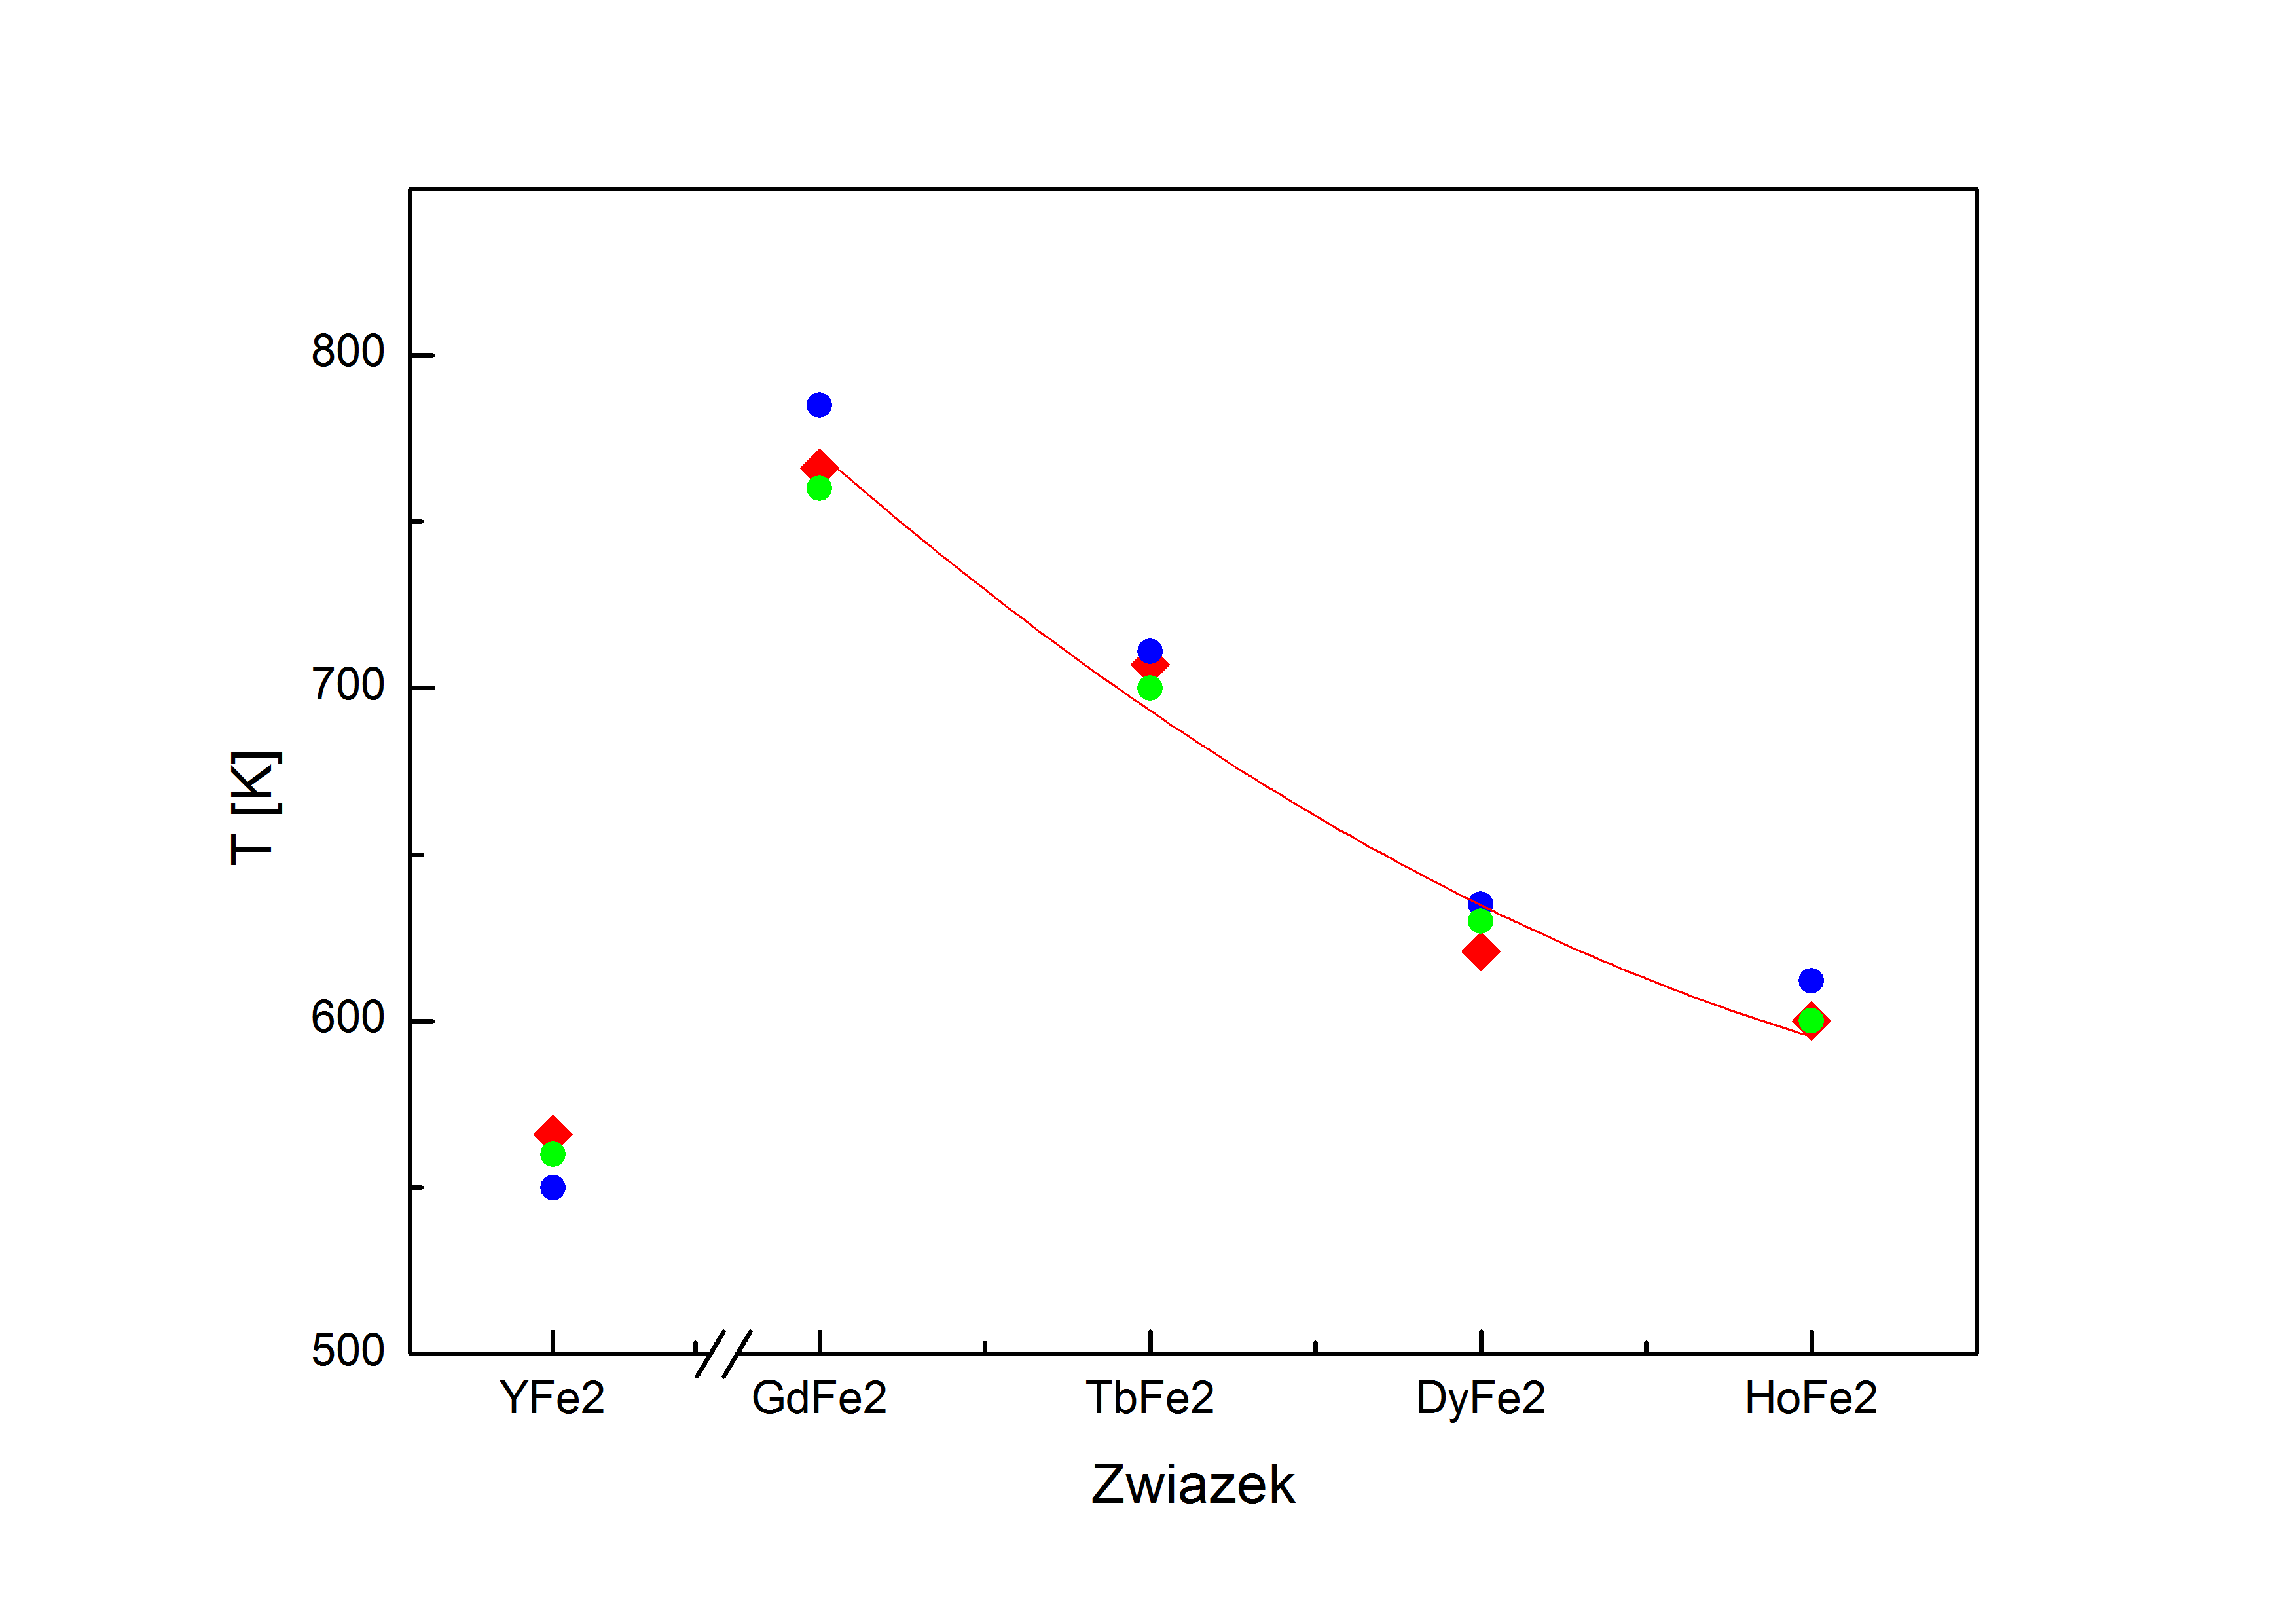
\includegraphics[width =1.0\textwidth]{../img/TempCurie1}
    \caption{Temperatura Curie badanych związków}
    \label{RysTempCurie}
\end{figure}

Do danych z wykresu dopasowano krzywą o równaniu ogólnym 

  \begin{equation}
   y=a_2x^2+a_1x+a_0
    \label{parabola}
  \end{equation}

Wyliczone za pomocą progamu OriginPro równanie ma postać

  \begin{equation}
   T_C=9,5x^2-124,9x+982,4 [K]
    \label{gotowaParabola}
  \end{equation}







\end{document}